%#!platex jou.tex

\chapter{文章の書き方}\chaplab{kousei}

\begin{abstract}
{\LaTeX}で文書を作成するためには文章の組版に関する約束事を
知る必要があります.論理的な文章を書きたいと思ったら,その理
論を知る必要があります.この章ではそれらを{\LaTeX}で実現する
ための基本的な部分を説明します.
\end{abstract}

%\section{文章の構造}
%
%簡単な文書を作成するうえで覚えたほうが良い項目を示します.
%\begin{description}
%\item[表 題] 
%   文書には必ず表題をつけて\K{誰}が\K{いつ},\K{何}を
%   作成したのかを示します.
%\item[目 次] 
%   ページが多い場合には目次をつけて読者に参照しや
%   すいようにします. 
%\item[見出し]
%   見出しを付けてこれから何について話をするのかを
%   明確にします. 
%\item[字下げ] 
%   段落始めは1文字ほど開けます.
%\item[段 落] 
%   一つの話題について一区切り付いたら段落を分けます.
%\item[句読点] 
%   文章の中で文の区切り,文の終わりには句読点などの区切り記号を
%   付けます.
%\item[注 釈] 
%   難解と思われる用語,補足すべき情報があれば注釈
%   として添えます.
%\end{description}
%
%これは日本語でもほかの言語でもほぼ共通だと思います.
%誰かに何かを文書で伝えるときにこれらの要素は必要でしょう.
%文書の最小構成単位は\yo{単語}です.\yo{文字}から\yo{文}ができ,
%\yo{段落}ができ\yo{節}ができ,\yo{章},\yo{部}へとつながって
%いきます.日本語の場合は表意文字なので最小単位は\yo{1文字}
%に相当します.
%
%{\LaTeX}はユーザが約束通りにコマンドを打ち込み文章を
%練り上げていれば,字下げ,相互参照,図表の配置,目次の作成な
%ど様々なことを半自動的に行ってくれます.ここではその基本的な
%約束を紹介します.

\section{文章の論理構造}
一般的な\Z{文書}\ (\Z{document}) を作成するうえで覚えたほうが
良い項目を示します.
\begin{description}
\item[表 題 (\Z{title})]
   文書には必ず\Z{表題}をつけて\K{誰}\ (\C{author}) が\K{いつ}\ 
   (\C{date}),\K{何}\ (\C{title}) を作成したのかを示します.
\item[目 次 (\Z{contents})]
   ページが多い場合には\Z{目次}をつけて読者が参照しや
   すいようにします.大規模な文書の場合,読者はまず目次を参照し,
   その文書を読むべきかどうかを判断しますので,\Z{学位論文}などでは
   目次は必須項目です.
\item[見出し (\Z{headline})]
   \Z{見出し}を付けてこれから何について話をするのかを明確にします.
   見出しは目次と関連していますので,読者がすぐに理解できるように
   します.
\item[段 落 (\Z{paragraph})]
   一つの話題について一区切り付いたら\Z{段落}を分けます.
\item[字下げ (\Z{indentation})]
   段落始めは全角1文字ほど開けて\Z{字下げ}を行ないます.
   欧文の場合,見出し直後の字下げは慣習的に行ないません.
\item[句読点 (\Z{punctuation})]
   \indindz{記号}{文を区切る}%
   文章の中で文の区切り,文の終わりには\Z{句読点}などの区切り記号を
   付けます.
\item[注 釈 (\Z{note})]
\index{難解な用語}%
\index{補足情報の追加}%
   難解と思われる\Z{用語},補足すべき\Z{情報}があれば\Z{注釈}として添えます.
   注釈はあくまで補足情報であって,読者がその注釈を読まなくても,
   何ら影響がないようにします.
\end{description}
このような構造は日本語や他の言語でもほとんど共通です.
誰かに何かを文書で伝えるときにはこのような構造が必要になります.
文書の最小構成単位は\KY{単語} (\Z{word}) です.\KY{文字} 
(\Z{character}) から\KY{文} (\Z{sentence}) ができ,
\KY{段落} (\Z{paragraph}) ができ,\KY{節} (\Z{section}) ができ,
\KY{章} (\Z{chapter}),\KY{部} (\Z{part}) へとつながって
いきます.日本語は漢字や仮名文字がありますが最小単位は\KY{文字} (\Z{letter})
に相当します.
\begin{table}[htbp]
 \begin{center}
  \caption{文書の構成要素}\label{tab:kouzou}
  \begin{tabular}{*7c}
   \TR
\Th{文字} & \Th{単語} & \Th{文} & \Th{段落} & \Th{節} & \Th{章} & \Th{部}\\
   \MR
   letter & word & sentence  & paragraph & section & chapter  & part \\
   \BR
  \end{tabular}
 \end{center}
\end{table}

{\LaTeX}はユーザが約束通りにコマンドを打ち込み文章を
練り上げていれば,字下げ,相互参照,図表の配置,目次の作成など,
様々な事を半自動的に行ってくれます.%ここではその基本的な
%約束を紹介します.
この章では\LaTeX におけるそれらのルールについて解説します.


\section{表題}\seclab{maketitle}

%\Z{表題}はその文書が何について書かれたものなのかを示すために
%必要な要素です.通常は\yo{題名},\yo{作者},\yo{日付}を書くのが
%一般的ですからプリアンブルに
\zindind{表題}{の役割}%
{表題}はその文書が何について書かれたものなのかを示すために
必要な要素です.通常は\KY{題名} (\Z{title}),\KY{作者} (\Z{author}),
\KY{日付} (\Z{date}) を書くのが
一般的ですからプリアンブルに次の三つを書き込みます.
\begin{Syntax}
\begin{tabular}{*3l}
\C{title}\pa{題名} & \C{author}\pa{作者} & \C{date}\pa{日付}\\
\end{tabular}
\end{Syntax}
{\LaTeX}ではプリアンブルに表題の情報を
書き込んでも出力まではしませんので\verb|\begin{document}|
の後に
\begin{Syntax}
 \Cmd{maketitle}
\end{Syntax}
とします.

例として入力が以下に示すようなものだと仮定します.

\begin{InTeX}
\documentclass{jarticle}
\title{はじめての\LaTeX}
\author{未来 太郎}
\date{2004年3月30日}
\begin{document}
\maketitle
{\LaTeX}を使うのはこれが初めてです.
\end{document}
\end{InTeX}

大体の出力は以下のようになります.

\begin{OutText}
\begin{center}
{\LARGE \textbf{はじめての\LaTeX }}\\[1.5em]
{\large 未来 太郎}\\[.7em]
{2004年3月30日}\\[.7em]
\end{center}
\quad {\LaTeX}を使うのは$\ldots$
\end{OutText}

\begin{Exe} \exelab{maketitle1}\indindz{区切り}{著者の}%
著者が複数人いるときは \Cmd{and}を使って区切ります.
所属などがあるときは \Cmd{thanks}で欄外に出力します.
以下のようなソースを実際に自分で出力してみてください.
またその結果も吟味してください.

\begin{InTeX}
\author{夏目漱石\thanks{○○研究所 ○○事業部}  \and
        福澤諭吉\thanks{△△株式会社 △△研究所}\and
        芥川龍之介\thanks{□□大学 □□学部 □□学科}}
\end{InTeX}
\end{Exe}

\begin{Exe} \exelab{maketitle2}
もう少し派手に著者名を紹介するとき,例えば
\yo{氏名},\yo{所属},\yo{連絡先}の三つを記述したいときは
次のようにします.

\begin{InTeX}
\author{日本太郎\\ ○○大学 □□学科\\ name@server.ac.jp}
\end{InTeX}

このソースを実際に出力しその結果を吟味してください.
\exeref{maketitle1}の \cmd{thanks}命令と \cmd{and}命令を使います.

\begin{InTeX}
\author{夏目漱石\thanks{○○大学 ○○学科 name@server.ac.jp}}
\end{InTeX}

もしくは改行で区切る方法のどちらも試してください.

\end{Exe}

\begin{Prob}\label{prob:maketitle:and}
 以下のソースを出力してその結果を吟味してください.

\begin{InTeX}
\author{夏目漱石 \\  ○○研究所 \\ ○○事業部  \and
        福澤諭吉 \\  △△株式会社 \\ △△究所\and
        芥川龍之介\\ □□大学 □□学部 \\ □□学科}
\end{InTeX}

この場合は横に著者が並びますが\qu{\cmd{and}}を取り除いて
\qu{\texttt{\bs\bs}}に書き換えると出力はどう変わるでしょうか.
\end{Prob}

\begin{Exe}
クラスファイルによる表題の体裁では不都合があるとき,
その場しのぎ的には次のように調整します.

\begin{InTeX}
\begin{center}
{\LARGE \textbf{はじめての\LaTeX }}\\[2em]
{\large 未来 太郎}\\[1em]
{2004年3月30日}\\[1em]
\end{center} 
\end{InTeX}

本来はクラスファイル中の \C{maketitle} 周辺のコマンドを
適切に調整するのが望ましいでしょう.
\end{Exe}

\section{見出し}\zindind{見出し}{の作成}%
%文書に\KY{見出し}と\K{目次}がなければ,記事の検索
%に時間がかかるのは容易に想像できるでしょう.そこで,文書の中に
%は\K{階層的な見出し}を作成します.またその文書の概略
%が存在すればその文書に何が書かれているのかがすぐに分かるので,
%\K{概要}を付け足すのも効果的です.
文書に\KY{見出し} (\Z{sectioning}) と\K{目次} (\Z{contents}) がなければ,
\Z{記事の検索}に時間がかかるのは容易に想像できるでしょう.そこで,
文書の中には\K{階層的な見出し} (\Z{nested sections}) を作成します.
\zindind{文書}{の概略}%
またその文書の概略が存在すればその文書に何が書かれているのかがすぐ
に分かるので,\K{概要} (\Z{abstract})を付け足すのも効果的です.


\subsection{見出しの出力}\indindz{番号}{通し}%
文書の中の一連の段落に何が書かれているのかを分かりやすくするために
見出しを記述します.また見出しは同一ページに同じ名前のものが存在し
ても良いように通し番号をつけて\Z{一意}的に管理します.

{\LaTeX}での見出しの定義は\tabref{headline}の通りです.%

\begin{table}[htpb]
 \begin{center}
  \caption{{\LaTeX}での見出しの定義}\tablab{headline}
  \newcommand{\midasiopt}{\opa{目次用の見出し}\pa{見出し}}%
  \begin{tabular}{l|l}
   \TR
   \Cmd{part}\midasiopt          & 部\\
   \Cmd{chapter}\midasiopt       & 章${}^*$\\
   \Cmd{section}\midasiopt       & 節\\
   \Cmd{subsection}\midasiopt    & 項\pp{小節}\\
   \Cmd{subsubsection}\midasiopt & 目\pp{小小節}\\
   \Cmd{paragraph}\midasiopt     & 段落\\
   \Cmd{subparagraph}\midasiopt  & 小段落\\
   \BR
  \end{tabular}
%  \\${}^*$\Cls{article}や\Cls{jarticle}では定義されていません.
\\{\small${}^*$\Cls{article}や\Cls{jarticle}では定義されていません.}
 \end{center}
\end{table}
%\cmd{section}などの見出し命令を使って見出しを作成します.
%前後の空白の調節や改ページ,改行,書体の変更などはほぼ自動的に
%行われ,\KY{通し番号}が付加されます.
%\qu{\opa{短縮した見出し}}という任意引数がありますが,
%これは見出しが非常に長いときに,それを短縮した文字列を目
%次に書き出すようにします.別に長いときだけではなく,
%見出しと目次の文字列を別にしたいときなどにも使えるでしょう.使い方
%は簡単です.見出しを階層構造的に書き記せば,{\LaTeX}は自動で階層ご
%とに番号付けをします.例としては次のような通し番号が振られます
%\pp{正確には出力は異なります}.
 \cmd{section}などの見出し命令を使って見出しを作成します.
前後の空白の調節や改ページ,改行,書体の変更などはほぼ自動的に
行われ,\KY{通し番号} (\Z{serial number})が付加されます.
\zindind{目次}{用の見出し}%
\indindz{見出し}{目次用の}%
\qu{\opa{目次用の見出し}}という任意引数がありますが,
これは見出しが非常に長いときに,それを短縮した文字列を目
次に書き出すようにします.別に長いときだけではなく,
見出しと目次の文字列を別にしたいときなどにも使えるでしょう.使い方
は簡単です.見出しを階層構造的に書き記せば,{\LaTeX}は自動で階層ご
とに番号付けをします.例としては次のような通し番号が振られます.

\par\vskip.3em\noindent
\begin{minipage}[c]{.47\textwidth}
\begin{verbatim}
\chapter{特殊相対性理論}
  \section{歴史的背景}
\chapter{一般相対性理論}
  \section{電気学との関連}
    \subsection{電気の次元数}
\end{verbatim}
\end{minipage}%
\hspace{.05\textwidth}%
\begin{minipage}[c]{.47\textwidth}
{\Large \textbf{第1章 特殊相対性理論}}\\
{\large \textbf{1.1 歴史的背景}}\\
{\Large \textbf{第2章 一般相対性理論}}\\
{\large \textbf{2.1 電気学との関連}}\\
{\normalsize \textbf{2.1.1 電気の次元数}}
\end{minipage}%


\subsection{見出しの深さ}\zindind{見出し}{の深さ}%
\begin{table}[htpb]
\begin{minipage}{.55\linewidth}
\caption{見出しの階層}\tablab{sectiondepth}
\begin{tabular}{lll}
\TR
\Th{見出し} & \Th{命令}     & \Th{深さ}${}^*$\\%$ 
\MR
部     & \Cmd{part}         & -1 \pp{0} \\
章     & \Cmd{chapter}      & 0  \pp{なし} \\
節     & \Cmd{section}      & 1   \\
小節   & \Cmd{subsection}   & 2   \\
小小節 & \Cmd{subsubsection}& 3   \\
段落   & \Cmd{paragraph}    & 4   \\
小段落 & \Cmd{subparagraph} & 4   \\ 
\BR
\multicolumn{3}{c}{${}^*$ 括弧内は\cls{(j)article}での深さ}
\end{tabular} 
\end{minipage}
\begin{minipage}{.44\linewidth}
\hskip1zw 文章の論理構造を整理するとき,一つの文書を\K{項目ごと}に分ける
事ができます.さらにその項目を小項目で分ける事もでき
るわけです.小項目があると文書の構造は\K{階層的に}なります.
項目が分かれている事を区別するために見出しを付けます.
見出しを\Z{目次}としてひとまとめに出力すると,読者は
目的の項目を探しやすくなります.\par
\end{minipage}
\end{table}
%{\LaTeX}ではあらかじめ部,章,節,小節,小小節,段落,小段落
%という七つの見出し用のコマンドを用意しています.
%ただし\cls{(j)article}などで章は用意されていませんし,
%クラスによって深さが若干違います. 
{\LaTeX}ではあらかじめ
部 (\Z{part}),
章 (\Z{chapter}),
節 (\Z{section}),
小節 (\Z{subsection}),
小小節 (\Z{subsubsection}),
段落 (\Z{paragraph}),
小段落 (\Z{subparagraph})
という七つの見出し用のコマンドを用意しています.
ただし\cls{(j)article}などで章は用意されていませんし,
クラスによって深さが若干違います. 


\section{目次の出力}
%\Z{目次}は見出しから読みたい箇所に移動するための見出し一覧です.
%これは20ページ以上の文書には必須でしょう.目次といっても{\LaTeX}では
%\begin{Syntax}
%\Cmd{tableofcontents}
%	    \pp{\K{目次}を出力するための命令}\\
%\Cmd{listoffigures} \indindz{目次}{図}
%    	    \pp{\KY{図目次}を出力するための命令}\\
%\Cmd{listoftables} \indindz{目次}{表}
%    	    \pp{\KY{表目次}を出力するための命令}
%\end{Syntax}
%の三つの命令が用意されており,それぞれ出力したい場所に命令を書きます.
%注意すべきこととして目次を作成するためには最低2回のタイプセットをし
%ます.
\Z{目次}は見出しから読みたい箇所に移動するための\KY{見出し一覧}です.
これは数十ページ以上の文書に存在する事が望まれます.目次といっても
{\LaTeX}には次の三つの命令が用意されています.

\begin{Syntax}
\indindz{目次}{図}%
\indindz{目次}{表} %
\begin{tabular}{ll}
 \C{tableofcontents} & 
    \pp{\KY{目次} [\Z{Contents}] を出力するための命令}\\
 \C{listoffigures} &
    \pp{\KY{図目次} [\Z{List of Figures}] を出力するための命令}\\
 \C{listoftables} &
    \pp{\KY{表目次} [\Z{List of Tables}] を出力するための命令}
\end{tabular}
\end{Syntax}

目次を表示するためには,それぞれ出力したい場所に命令を書きます.
注意すべき事として,
\K{目次を作成するためには最低2回のタイプセットを行います}.

その理由を考えるために,以下のようなファイル\fl{mokuji.tex}を作ります.

\begin{InTeX}
\documentclass{jarticle}
\begin{document}
\tableofcontents%目次を出力する命令
\section{序論}
\subsection{研究背景}
\section{手法}
\subsection{実験環境}
\end{document}
\end{InTeX}

次にこのファイル\fl{mokuji.tex}をタイプセットすると
出力ファイル\fl{mokuji.dvi}にはただ\yo{目次}と出力されるだけで,
実際の目次が出力されていない事に注目してください.
コンソールには次のようなメッセージが表示されます.

\begin{OutTerm}
 No file mokuji.aux.
 No file mokuji.toc.
 [1] (./mokuji.aux) )
\end{OutTerm}
\Exten*{aux}%

\dos{No File なんとか} という
のは\va{なんとか}というファイルが存在しない,足りないという
メッセージです.ですが,同じディレクトリ\pp{フォルダ}には
\fl{mokuji.aux}も\fl{mokuji.toc}も存在するようです.どうやら
タイプセットする前には存在せず,タイプセット後にこの二つのファイルは
作成されたようです.この二つのファイルを覗いてみましょう.まずは%
\indindz{ファイル}{中途}中途ファイル\fl{mokuji.aux}には
次のように,ちょっと分かりづらい記述があります.

\begin{InTeX}
\relax
\@writefile{toc}{\contentsline{section}{\numberline{1}序論}{1}}
\@writefile{toc}{\contentsline{subsection}{\numberline{1.1}研究背景}{1}}
\@writefile{toc}{\contentsline{section}{\numberline{2}手法}{1}}
\@writefile{toc}{\contentsline{subsection}{\numberline{2.1}
   実験環境}{1}} 
\end{InTeX}

要するに%
\indindz{ファイル}{目次用の}%目次ファイル
\fl{mokuji.toc}に見出し関係の記述をどうすべきかを書いているようです.
さらに目次用の中途ファイル\fl{mokuji.toc}には
先ほどの\fl{mokuji.aux}とほとんど同じ記述があります.

\begin{InTeX}
\contentsline{section}{\numberline{1}序論}{1}
\contentsline{subsection}{\numberline{1.1}研究背景}{1}
\contentsline{section}{\numberline{2}手法}{1}
\contentsline{subsection}{\numberline{2.1}実験環境}{1} 
\end{InTeX}

これを踏まえてもう1度\fl{mokuji.tex}をタイプセットします.
するとコンソールには次のようなメッセージが表示されます.

\begin{OutTerm}
(d:/usr/local/share/texmf/ptex/platex/base/jarticle.cls
Document Class: jarticle 2004/02/25
) (./mokuji.aux) (./mokuji.toc) [1] (./mokuji.aux) )
\end{OutTerm}

どうやら\fl{mokuji.aux}も
\fl{mokuji.toc}も存在し,それらを適切に処理してくれたようです.
出力ファイル\fl{mokuji.dvi}の先頭には始め出力されなかった\yo{目次}
がある事でしょう.

\begin{OutText}
{\large\headfont 目次}\\[1zw]{\small
\hbox to 5zw{\textbf{1}\hfil}\textbf{序論}\hfill 1\\
\hskip2zw\hbox to 3zw{1.1\hfil}研究背景\dotfill~1\\
\hbox to 5zw{\textbf{1}\hfil}\textbf{手法}\hfill 1\\
\hskip2zw\hbox to 3zw{1.1\hfil}実験環境\dotfill~1}
\end{OutText}

\subsection{目次を出力する深さ}
\index{目次!tocdepth@\texttt{tocdepth}}%
\zindind{目次}{の深さ}%
%\index{カウンタ!tocdepth@\texttt{tocdepth}}%
目次をどの階層まで出力するかはカウンタ\Kount{tocdepth}の
値を\tabref{sectiondepth}に従って変更します.
\cls{jsbook}などで章\pp{\cmd{chapter}}まで出力したいならば
次のようにします.

\begin{InTeX}
\secounter{tocdepth}{0}
\end{InTeX}

\cls{(j)book}と\cls{(j)report}の標準は2,
\cls{(j)article}ならば3です.\cls{jsbook}は1になっています.

\subsection{見出しの番号付けの深さ}
\zindind{見出し}{の通し番号}%
\zindind{番号}{の深さ}%
\index{目次!secnumdepth@\texttt{secnumdepth}}%
\zindind{目次}{の番号付けの深さ}%
%\index{カウンタ!tocdepth@\texttt{secnumdepth}}%
見出しの通し番号はカウンタ\Kount{secnumdepth}によって
どの階層まで出力するかを決められます.\kount{secnumdepth}の
値は\tabref{sectiondepth}に従って変更します.
小節\pp{\cmd{subsection}}までに番号を付けるようにするには
次のようにします.これは目次側にも影響します.

\begin{InTeX}
\setcounter{secnumdepth}{2}
\end{InTeX}



\section{概要の出力}
%文書の概略が存在すればその文書に何が書かれているのかが大まかに
%分かるので\Z{概要}を書くのが良いでしょう.
%%さすがに1ページの文書には必要ないでしょうが.
%\yo{概要}は\yo{はしがき}とも呼ばれ,文書クラスによって
%出力方法が違います.\cls{(j)article}系ならば
%\Env{abstract}環境を使います.この\env{abstract}環境
%は \Cmd{maketitle} 命令と関わりがあるので概要を出力するために
%は \cmd{maketitle} 命令の後に書きます.
文書の概略が存在すればその文書に何が書かれているのかが大まかに
分かるので\Z{概要} (\Z{abstract}) を書くのが良いでしょう.
%さすがに1ページの文書には必要ないでしょうが.
\yo{概要}は\yo{はしがき}とも呼ばれ,文書クラスによって
出力方法が違います.\cls{(j)article}系ならば
\Env{abstract}環境を使います.この\env{abstract}環境
は \Cmd{maketitle} 命令と関わりがあるので概要を出力するために
は \cmd{maketitle} 命令の後に書きます.
\begin{Syntax}
\cmd{maketitle}\\
\verb|\begin{abstract}|\\
\va{文書の概要}\\
\verb|\end{abstract}|
\end{Syntax}
次に\cls{(j)report}の場合ですが概要専用の環境は用意されてい
ません.そこで概要を\Z{章立て}すると良いので \Cmd{chapter*} 
命令を使います.このとき \cmd{chapter}命令にアスタリスク 
\qu{\texttt*}を付けると目次に見出しを書き出さず,章番号を付け足しません.
例として次の記述をしてから概要の文章を書きます.

\begin{InTeX}
\chapter*{概要}\addcontentsline{toc}{chapter}{概要}
\end{InTeX}

標準の文書クラスでは
概要専用のコマンドは定義されていません.用途は異なりますが
\Hito{奥村}{晴彦}の\Cls{jsbook}には\env{abstract}環境が定義
されています.これは各章の始めに\yo{この章について}のような
\kenten{まえがき}を書くときに使われます.

%最後に\cls{(j)book}場合ですが,これは \Cmd{frontmatter}が宣言
%されているときに \cmd{chapter}命令を使うと良いと思います.
%具体的には\index{まえがき}%
%\begin{InTeX}
%\begin{document} 
%\frontmatter % 前付け
%\chapter{まえがき}
%ここに概要やまえがきを書きます.
%\mainmatter % 本文
%\chapter{序論}
%\end{InTeX}
%とすると目次に概要を書き出しますが番号を付け足しません.

最後に\cls{(j)book}の場合ですが,これは \Cmd{frontmatter} が宣言
されているときに \cmd{chapter}命令を使うと余計な手間を省く事ができます.
具体的には\index{まえがき}%
次のようにすると目次にも概要を番号なしで書き出します.

\begin{InText}
\begin{document} 
\frontmatter%前付け
\chapter{まえがき}
ここに概要やまえがきを書きます.
\mainmatter%本文
\chapter{序論}
\end{InText}






\section{段落と字下げ}\indindz{字下げ}{段落始めの}%
文章で段落をはじめようと思えば,まず\KY{字下げ} (\Z{indentation}) 
をします.%小学校の作文でも必ず作文用紙
%では次の段落に移るときは1文字開けたと思います.
この字下げの作業を{\LaTeX}は半自動で行います.使い方は
1行空けて入力すれば良いだけです.

\begin{InText}
天皇は、日本国の象徴であり日本国民統合の象徴であつて、
この地位は、主権の存する日本国民の総意に基く。 

皇位は、世襲のものであつて、国会の議決した皇室典範の
定めるところにより、これを継承する。 

天皇の国事に関するすべての行為には、内閣の助言と承認
を必要とし、内閣が、その責任を負ふ。 
\end{InText}

%これにより次のような出力が得られます.

\begin{OutText}
\hskip1zw 天皇は、日本国の象徴であり日本国民統合の象徴であつて、
この地位は、主権の存する日本国民の総意に基く。 \par
\hskip1zw 皇位は、世襲のものであつて、国会の議決した皇室典範の
定めるところにより、これを継承する。 \par
\hskip1zw 天皇の国事に関するすべての行為には、内閣の助言と承認
を必要とし、内閣が、その責任を負ふ。 
\end{OutText}

このように自動的に字下げがなされます\footnote
   {『日本国憲法』 1947年5月3日\,施行の第1条から第3条までの引用.}.
明示的に \Cmd{par}命令
で段落の終了を知らせる事ができ,以下のようにも書けます.

\begin{InText}
天皇は、日本国の象徴であり日本国民統合の象徴であつて、
この地位は、主権の存する日本国民の総意に基く。\par
皇位は、世襲のものであつて、国会の議決した皇室典範の
定めるところにより、これを継承する。\par
天皇の国事に関するすべての行為には、内閣の助言と承認
を必要とし、内閣が、その責任を負ふ。\par
\end{InText}

\latexno{とワープロの違い}%
\indindz{改行}{原稿における}%
\indindz{改行}{出力結果における}%
\zindind{原稿}{中の改行}%
以上のように{\LaTeX}はワープロソフトとは違い,\K{原稿中の一つ
の改行が出力と対応していない}のがお分かりになるでしょう.
{\LaTeX}では{改行}すべき位置を自動で計算しているのです.

\begin{Trick}
\indindz{幅}{字下げの}%
字下げの幅は \Cmd{parindent} という長さ変数で指定できます.
`\verb|\parindent = 3zw|'のようにすると約全角3文字分の字下げを段落の始め
で行う事ができます.
\end{Trick}



\subsection{行頭の字下げ}\seclab{indentfirst}
\zindind{字下げ}{の抑制}%
\zindind{行頭}{の字下げ}%
\indindz{字下げ}{行頭の}%

段落の開始には字下げをすべきなのですが,
何らかの理由により字下げを抑制したいときがあります.
字下げの有無に関しては \Cmd{indent} と \Cmd{noindent} 
命令が使えます.
\begin{Syntax}
\begin{tabular}{ll}
 \C{indent}   &(可能ならば字下げをします)\\
 \C{noindent} &(可能ならば字下げをしません)
\end{tabular}
\end{Syntax}
\cls{jreport}などのクラスファイルではこのような命令を
使っても行頭の字下げができないときがあります.
その場合は\Sty{indentfirst}パッケージを読み込みます.
\begin{InOut}
\usepackage{indentfirst}
\noindent 私は\indent 大学生ですか
ら,そうなります.\par
\noindent そうなりました.
\end{InOut}

\zindind{字下げ}{の幅の調節}%

\begin{Prob}
行頭の字下げをせずに段落と段落に\Z{空き}を入れて段落の終わりと段落の始ま
りを示すという事を{\LaTeX}で行うためには,段落と段落の空きを調節す
る \C{parskip}という可変の長さ変数を調節します.

\begin{InTeX}
\parindent = 0pt % 字下げ
\parskip = 10pt plus 0pt minus 0pt
\end{InTeX}

実際にこのような設定にすれば分かりますが,
ありとあらゆる部分に空きを挿入しますので,その出力結果を吟味してください.
\end{Prob}


\subsection{段落の字下げ\zdash\Y{indent}}

\indindz{引用}{文の}%
\indindz{字下げ}{段落の}%
文を引用している場合はそれが\Z{引用}である事を明確に
するために,段落全体を字下げする習慣があります.
これには\Env{quote}環境や\env{quotation}環境が
使えます.ただしこの場合は自分で字下げ幅を
設定できません.%\env{quote}環境の中で使われている
%\Env{list}環境を自分でカスタマイズするとうまく行きます.
簡単に段落の字下げを調整するには\Sty{indent}\footnote{\CTAN{macros/latex209/contrib/misc/indent.sty}}パッケージの\Env{indentation}環境を使います.

\begin{Syntax}
 \verb|\begin{indentation}|\pa{左側の字下げ}\pa{右側の字下げ}\\
 \va{文章内容}\\
 \verb|\end{indentation}|
\end{Syntax}

\env{indentation}環境の\K{一つ目}の必須引数には
\K{左側の}字下げ,\K{二つ目}には\K{右側の}字下げを指定します.
\begin{InOut}
ここは普通の文章領域です.不必要
に字下げを調整するのは好ましいこ
とではありません.
\begin{indentation}{3zw}{3zw}
左側の字下げは全角3文字分,右側の
字下げも全角3文字分ありますか?
\end{indentation}
\begin{indentation}{0zw}{5zw}
左側の字下げはなし,右側の字下げ
は全角5文字分ありますか?
\end{indentation}
ここも普通の文章領域です.
\end{InOut}


\subsection{ダブルスペース}\seclab{doublespace}

%また\Z{ダブルスペース}といって\KY{行送り}を倍にする
%ということも迫られる場合があるようです.
%%\pp{2行取りって言うのかな?}
%これは行送りの量を決める長さ変数 \Cmd{baselinestretch} を
%\begin{InTeX}
%\renewcommand{\baselinestretch}{2}
%\end{InTeX}
%とする方法があります.他にも\Sty{doublespace}パッケージを
%\begin{InTeX}
%\usepackage{doublespace} 
%\end{InTeX}
%としてプリアンブルで読み込むと上記の方法よりもうまく
%ダブルスペースを実現できます.


\Z{ダブルスペース}といって\KY{行送り}を倍にするという事を
迫られる場合があります.
%これは行送りの量を決める長さ変数 \Cmd{baselinestretch} を
%\begin{InText}
%\renewcommand{\baselinestretch}{2}
%\end{InText}
%とする方法があります.
%他にも\Sty{doublespace}パッケージを
%\begin{InText}
%\usepackage{doublespace} 
%\end{InText}
%としてプリアンブルで読み込むと上記の方法よりもうまく
%ダブルスペースを実現できます.
これには \person{Geoffrey}{Tobin}による\Y{setspace}パッケージ
を使う事が考えられます\footnote{他にも \Y{doublespace}パッケージ
を使う方法や \Cmd{baselinestretch} 命令を再定義する方法もあります.}.
\begin{Syntax}
\begin{tabular}{ll}
 \C{singlespacing}   &(通常通りの行送りに設定する)\\
 \C{onehalfspacing}  &(通常の1.5倍の行送りにする)\\
 \C{doublespacing}   &(通常の2倍の行送りにする)\\
\end{tabular}\\
 \verb|\begin{spacing}|\pa{数値} \va{文章} \verb|\end{spacing}|
\end{Syntax}
\va{数値}を指定して行送りを変更できる\Env{spacing}環境も用意されています.%
\begin{InOut}
\usepackage{setspace}
\singlespacing
ここは通常の\par 行間\par
\doublespacing
ここは通常の\par 2倍の行間\par
\begin{spacing}{.8}
ここは通常の\par 0.8倍の行間\par
\end{spacing}
\end{InOut}



\section{長さの単位}\index{単位}

%先ほどは何らかのパラメータに数値を代入する
%\begin{InTeX}
%\parindent=0pt 
%\end{InTeX}
%のような記述がありました.これにはポイント
%\qu{pt}という単位が使われています.
%{\LaTeX}において使用できる\zindind{長さ}{の単位}長さの単位
%\pp{\tabref{latexunit1}}は色々あります.ポ
%イントは絶対的な長さではないのでクラスファイ
%ルによって変わったりプログラムによっても若干
%の違いがあります.
%\begin{table}[htbp]
%\begin{center}\indindz{幅}{Mの字の}\indindz{高さ}{xの字の}%
%\caption{{\LaTeX}で使用できる主な単位}\tablab{latexunit1}
%\begin{tabular}{cll}
%\TR
%\Th{単位}& \Th{読み}&  \Th{補足}\pp{数値は概算}\\
%\MR
%in& インチ             & 1\,in $=$ 25.4\,mm $=$ 72.27\,pt \\
%cm& センチメートル      & 1\,cm $=$ 10\,mm $=$ 28.3\,pt \\
%mm& ミリメートル        & 1\,mm $=$ 2.83\,pt \\
%pt& ポイント           & 1\,pt $=$ 0.35\,mm\\
%em& Mの字の幅と同じ.  & 使用中のフォントに依存 \\
%ex& xの字の高さと同じ.  & 使用中のフォントに依存  \\
%zw& 日本語の一文字の幅.& 使用中のフォントに依存  \\
%\BR
%\end{tabular}
%\end{center}
%\end{table}
%\Hito{奥村}{晴彦}の\cls{jsclasses}ではクラスオプションに
%\Option{10pt}以外のフォントサイズ指定がされている場合は
%版面の拡大縮小を使っていますので単位がずれます.これには
%各単位に\qu{\str{true}}を付けて長さを指定します.例えば
%\qu{\str{cm}}ならば\qu{\str{truecm}}のようにします.
%%このようにすると\Cmd{magstep}の影響がありません.
%%↑はいらないよなぁ.

\subsection{\LaTeX での単位の取り決め}
\latexno{における単位}
\index{数値の代入}%

\index{=@\str{=}!代入としての\zdash}%
\index{=@\str{=}}%
先ほどは何らかの\Z{変数}(\Z{パラメータ})に数値を代入する時に
`\verb|\parindent=0pt |'
という記述がありました.これにはポイント
\qu{pt}という単位が使われています.
{\LaTeX}において使用できる\zindind{長さ}{の単位}長さの単位
\pp{\tabref{latexunit1}}は色々あります.ポイントは%
\indindz{長さ}{絶対的な}%
\Z{絶対的な長さ}ではないのでクラスファイルによって変わった
りプログラムによっても若干の違いがあります.
\begin{table}[htbp]
\begin{center}
\indindz{幅}{Mの字の}%
\indindz{高さ}{xの字の}%
\zindind{日本語}{の幅}%
\caption{{\LaTeX}で使用できる主な単位}\label{tab:latexunit1}
\begin{tabular}{c*3l}
\TR
\Th{単位}& \Th{読み}&  \Th{補足\pp{数値は概算}} & \Th{実際の長さ}\\
\MR
in& \Z{インチ}  &1\,in $=$ 25.4\,mm $=$ 72.27\,pt & \demowidth{1truein}\\
cm& \Z{センチメートル} &1\,cm $=$ 10\,mm $=$ 28.3\,pt    & \demowidth{1truecm}\\
mm& \Z{ミリメートル}   &1\,mm $=$ 2.83\,pt           & \demowidth{1truemm}\\
pt& \Z{ポイント}      &1\,pt $=$ 0.35\,mm           & \demowidth{1truept}\\
em& Mの字の幅と同じ. &使用中のフォントに依存    & \demowidth{1em}\\
ex& xの字の高さと同じ.&使用中のフォントに依存  & \demowidth{1ex}\\
zw& 日本語の一文字の幅.&使用中のフォントに依存   & \demowidth{1zw}\\
\BR
\end{tabular}
\end{center}
\end{table}
\hito{奥村}{晴彦}の\cls{jsclasses}ではクラスオプションに
\Option{10pt}以外のフォントサイズ指定がされている場合は%
\zindind{紙面}{の拡大縮小}%
\zindind{単位}{のずれ}%
紙面の拡大縮小を使っていますので単位がずれます.これには
各単位に\qu{\str{true}}を付けて長さを指定します.例えば
\qu{\str{cm}}ならば\qu{\str{truecm}}のようにします.
%このようにすると \Cmd{magstep}の影響がありません.
%↑はいらないよなぁ.

\subsection{単位の使い方}
\indindz{記号}{単位}%
\Z{単位}は基本的に\Z{国際単位}\Z{SI}に従いローマン体,
記号はイタリック体で表記します.\zindind{単位}{の接頭語}%
単位の\Z{接頭語}として\tabref{SI:prefix}の\Z{修飾子}が
使用できます\footnote{この他にも$10^{24}$から$10^{-24}$まで
 (Y Z P T G M k m \textmu\ n p f a z y) ありますが,頻繁に用いられるだろ
 う修飾子だけを掲載しました.}.

\begin{table}[htbp]
 \begin{center}
  \caption{SIの基本単位}\label{tab:SI:base}
 \begin{tabular}{llllll}
 \TR
 \Th{名称} & \Th{英語名称} & \Th{記号} & \Th{単位} & \Th{読み} & \Th{英語読み}\\
 \MR
 \Z{長さ}  & \Z{length}& $l$  & m    & \Z{メートル}  & \Z{meter}\\
 \Z{質量}  & \Z{mass}  & $m$  & kg   & \Z{キログラム}& \Z{kilogram}\\
 \Z{時間}  & \Z{time}  & $t$  & s    & \Z{秒}        & \Z{second}\\
 \Z{物理量}& \Z{amount of substance} & $n$ & mol  & \Z{モル}      &\Z{mole}\\
 \Z{電流}  & \Z{electric current}    & $I$ & A    & \Z{アンペア}  &\Z{ampere}\\
 \Z{熱力学温度}& {thermodynamic} 
      &$T$&K & \Z{ケルビン}  &\Z{kelvin}\\
          &  temperature & & & \\
 \Z{光度} & \Z{luminous intensity}  & $I$ & cd   & 
      \Z{カンデラ}  &\Z{candela}\\
 \BR
 \end{tabular}
 \end{center}
\end{table}
%
\begin{table}[htbp]
\newcommand*\DP[1]{$10^{#1}$}
 \begin{center}
  \caption{$10^n$の修飾子}\label{tab:SI:prefix}
  \begin{tabular}{*{15}{l}}
\TR
$10^n$&\DP{12}&\DP{9}&\DP{6}&\DP{3}&\DP{-3}&\DP{-6}&\DP{-9}&\DP{-12}\\
\MR
記号  & T & G & M & k & m & \textmu & n & p \\
名称  & \Z{テラ} & \Z{ギガ} & \Z{メガ} & \Z{キロ} & \Z{ミリ} & \Z{マイクロ}{*} & \Z{ナノ} & \Z{ピコ} \\
英語名称& \Z{tera} & \Z{giga} & \Z{mega} & \Z{kilo} & \Z{milli} & \Z{micro} & \Z{nano} & \Z{pico} \\
\BR
  \end{tabular}
\par\vskip1ex
\begin{footnotesize}
{*} ローマン体のマイクロ (\textmu) を出力するには
\Y{textcomp}パッケージの \cmd{textmu} コマンドを使います.
\end{footnotesize}
 \end{center}
\end{table}
%
\begin{InOut}
数値と単位の間には半角程度の空白を挿入
します.3\,mkg(3ミリキログラム)など,
修飾子を複数表記してはいけません.
3\,mkg (×) は正しくは3\,gとなります.
\end{InOut}
\indindz{空白}{数値と単位の}%
数値と単位の間には\K{半角程度の空白を挿入します}.
単位とその修飾子は\K{いかなる場合でもローマン体とします}.
\zindind{強調}{の中の単位}%
強調部分に単位が含まれる場合でも同様です.


\section{句読点}
\indindz{点}{句読}%

句読点は,文を区切るために文間に挿入する記号です.
\index{.@\verb+.+(句点)}\index{,@\verb+,+(読点)}%
\KY{句読点} (\Z{punctuation}) は組み方向を縦書きにするか横書きに
するかでも違います.%縦書きのときは何も迷わずに全角の\Z{読点}\yo{、}
%と\Z{句点}\yo{。}を用います.
\indindz{コンマ}{全角の}%
\indindz{ピリオド}{全角の}%
レポート・論文の多くは横書きの場合ですから,全角の
コンマ`,'とピリオド`.'を使うと良いでしょう.ただし,
欧文中心の文や段落にはすべて半角の句読点や括弧を使います.
\begin{InOut}
The length of a pen should be 
comrotable to write with: too long 
and it makes him tired; too short 
and it\ldots.\par Prof.~Albert 
Einstein (1897--1955) was born in 
German (see fig.~3).
\end{InOut}
欧文において,\Z{コロン},\Z{セミコロン}などの記号は\Z{コンマ},
\Z{ピリオド}と同様に,記号の前に空白(空き)を入れず,後ろに半角
の空白を挿入しています.
\index{:@\str{:}}
\index{;@\str{;}}

\Z{丸括弧}(\Z{パーレン})の左側(\Z{起こし})に空白を入れていますが,
右側(\Z{受け})には入れていません.

%\index{.@\verb+.+}\index{,@\verb+,+}%
%\Z{句読点}についてですが,縦書きにするか横書きにするかで
%違います.縦書きのときは何も迷わずに全角の\Z{読点}\yo{,}
%と\Z{句点}\yo{.}を用います.

横書きのときは句読点は\K{半角}のコンマとピリオドを使うのがベスト
だと思います.その場合は句読点の後には半角のスペースを入れてください.
横書きで全角の句読点を使うときは
\begin{OutText}
今日のお弁当のふたには``I wish I could.''という文句が書かれていた。
\end{OutText}
のように二つの文書に異なる句読点が混在する事になります.
なるべく句読点は統一したほうが気持ちが良いでしょう.
ただし,
\begin{OutText}
今日のお弁当のふたには「I wish I could。」という文句が書かれていた。
\end{OutText}
などとするのはとっても気持ち悪いのでやめたほうが無難です.
横書きのときは文章の内容と相談して句読点を決めてください.

句読点が少し気持ち悪く見える例です.
\begin{InOut}
地球は,青かった. 10\,m,高かった.
\end{InOut}

どのようにするのが良いかはご自分で判断していただければ良いのですが,
本書でも一応の見解を出しておきます.まずは欧文だけの場合を考え
ます.欧文のみの文書では以下の規則に従うだけで良いでしょう.
\begin{itemize}
 \item 句読点は半角のコンマ\yo{\str,}とピリオド\yo{\str.}を使う.
 \item 単語の\Z{引用}はシングルクオート\yo{\str{`'}},
   一文の引用はダブルクオート\yo{\str{`{}`{}'{}'}}を使う.
\end{itemize}
和文のみの場合は
\begin{itemize}
 \item 句読点は読点\qu{,}と句点\qu{.}を使う.
 \item 単語の引用は\Z{かぎ括弧}\qu{「」},
   文の引用は\Z{ダブルクオート}\qu{『』}を使う.
\end{itemize}
となるでしょう.ですが和文と欧文が混在する文書ではどのよう
に取り決めたら良いのでしょうか.本来ならばまず句読点のつけ
方も引用の仕方も一つの文書の中で統一するのが規則です.そのため
和文と欧文が混在する場合は欧文の規則に従うという事です.
%
ですが,そうすると別の問題が出てきます.日本語組版で
\yo{句読点は1文字分の幅を割り当てる}という規則に反す
る事があります.これには全角のコンマ\yo{,}とピリオド
\yo{.}を使うようにすると我慢できます.
%これは微妙なところなので,特に指定がなければ
%断腸の思いで欧文の規則に従うのが無難です.



\section{注釈}
%\Z{注釈}とは文章の中で出てきた注意すべき語句を説明するために
%付けるものです.注釈は読者が読まなくても良い,本文とは関係のない情報を
%示すために使われます.{\LaTeX}では2種類の注釈を出力できます.
%一つはページ下部に出力する\KY{脚注}\pp{\Cmd{footnote}},
%もう一つは注釈語の横に出力する\KY{傍注}%
%\marginpar{このように\K{傍注}が出力されます}
%\pp{\Cmd{marginpar}}です.
%紙面の下端に表示される脚注には \Cmd{footnote} 命令を使います.
%\begin{Syntax}
%注釈語\cmd{footnote}\pa{注釈内容}
%\end{Syntax}
%この命令を使用すると{\LaTeX}は組版時に自動的に \Cmd{footnote} で通し番号
%を付けます\footnote{このように注釈が文章の頁の下端に出力されます}.
%脚注の出力は使用しているクラスファイルによって違うので確認してみると
%良いでしょう.
%\begin{InOut}
%ラプラス変換やフーリエ変換\footnote{Fourier 
%Translation}は通常理工系の大学ならば必修で
%...と思われる.
%\end{InOut}

\zindind{注釈}{の役割}%
\Z{注釈} (\Z{note}) とは文章の中で出てきた注意すべき語句を
説明するために付けるものです.注釈は読者が読まなくても良い,
本文とは関係のない情報を示すために使われます.{\LaTeX}では
2種類の注釈を出力できます.
\zindind{注釈}{の位置}%
一つはページ下部に出力する\KY{脚注}\pp{\Cmd{footnote}},
もう一つは注釈語の横に出力する\KY{傍注}%
%\marginpar{このように\K{傍注}が出力されます}
\pp{\Cmd{marginpar}}です.
紙面の下端に表示される脚注には \Cmd{footnote} 命令を使います.
\begin{Syntax}
注釈語\cmd{footnote}\pa{注釈内容}
%注釈語\cmd{marginpar}\pa{注釈内容}
\end{Syntax}
レポート・論文の場合,\K{傍注を使わずに脚注のみを使うようにしてくださ
い}.

この命令を使用すると{\LaTeX}は組版時に自動的に \Cmd{footnote} で通し番号
を付けます\footnote{このように注釈が文章の頁の下端に出力されます.}.
脚注の出力は使用しているクラスファイルによって違うので確認してみると
良いでしょう.
\begin{InOut}
ラプラス変換やフーリエ変換\footnote
{Fourier Translation}は通常理工系の
大学ならば必修で\ldots と思われる.
\end{InOut}




\section{文字の強調}
\zindind{下線}{の意味}

ビジネス文書等では重要な文に\Z{下線} (\Z{underline}) を引いて
\Z{強調} (\Z{emphasis}) を表しているものがあります.
論文や書籍の場合は\K{欧文をイタリック体},\K{和文はゴシック体}にします.
\indindz{強調}{和文の}\indindz{強調}{文字列の}%
{\LaTeX}では文字列の強調のために \C{emph} 命令が使えます.
%もしかしたら使用している
%クラスファイルによっては和文がゴシック体になら
%ないかもしれません.
\begin{InOut}
欧文の強調には\emph{English 
Emphasize}として,和文の強調は
\emph{文字列の強調}のようにします.
\end{InOut}

%最近のワープロ文書では重要な文字列に\Z{下線}を引いて
%\Z{強調}を表現しているようです.論文や書籍では
%\K{欧文}を\K{イタリック体},\K{和文}の場合は
%\K{ゴシック体}にするほうが良いと思われます.
%\indindz{強調}{和文の}\indindz{強調}{文字列の}%
%{\LaTeX}では文字列の強調のために \cmd{emph} 
%が使えます.もしかしたら使用している
%クラスファイルによっては和文がゴシック体になら
%ないかもしれません.
%\begin{InOut}
%欧文の強調には\emph{English Emphasize}として,
%和文の強調は\emph{文字列の強調}のようにします.
%\end{InOut}

場合によっては \Cmd{em} コマンドが使えます.これは
\KY{宣言型コマンド}\pp{\secref{ml:command}}と
呼ばれるもので,広範囲な論理強調に使う事ができます.
ただしこのコマンドを使うならば\KY{イタリック補正}を
挿入する場合があります.イタリック補正とはイタリック体の
文字の直後にローマン体などの別のフォントが来た場合に
挿入すべき空白の事です.{\LaTeX}が用意している \Cmd{emph} 
や \Cmd{textit}などはこのイタリック補正
が適切に挿入されるようになっています.宣言型の強
調コマンド \Cmd{em}を使う場合は%
\glossary{"/@\hspace*{-1.2ex}\verb+"\/+}%"
自分で挿入しますから \cmd{/} 命令を使う事になります.%"
\begin{InOut}
\emph{Future University-Hakodate} 
is interesting.\par 
{\em FUN\/} is funky?\par
{\em FUN} is not funky?
\end{InOut}


\section{そのまま出力できない記号}
{\LaTeX}ではいくつかの半角の記号を直接出力する事ができません.
これは\Z{予約文字}と呼ばれるもので,\qu{\texttt\bs}に似た
命令の一種だと思ってください.出力できない記号は
\begin{quote}
 \verb+\ { } $ & # ^ _ ~ % < > |+
\end{quote}
の13個であり,それらの記号を出力するには\secref{chui}
を参照してください.
%%\glossary{?3@\hspace*{-1.2ex}\texttt{\protect\bs\#}\hskip1em(\#)}%\#
%%\glossary{?4@\hspace*{-1.2ex}\texttt{\protect\bs\%}\hskip1em(\%)}%\%
%%\glossary{?5@\hspace*{-1.2ex}\texttt{\protect\bs\$}\hskip1em(\$)}%\$
%%\glossary{?6@\hspace*{-1.2ex}\texttt{\protect\bs\&}\hskip1em(\&)}%\&
%%\glossary{yen@\hspace*{-1.2ex}\texttt{\protect\bs yen}\hskip1em(\yen)}%\yen
%%\glossary{?8@\hspace*{-1.2ex}\texttt{\protect\bs\_}\hskip1em(\_)}%\_
%\begin{table}[htpb]
%\begin{center}
%\caption{直接出力できない半角記号}\tablab{tokusyumoji}
%\begin{tabular}{ll|ll|ll}
%\{ & \verb|\{| & 
%\& & \verb|\&| & 
%\T{textgreater}\\
%\} & \verb|\}| &  
%\T{textbackslash} &  
%\T{textbar}  \\
%\# & \verb|\#| & 
%\yen & \verb|\yen|${}^*$ & 
%\T{textasciicircum} \\
%\$ & \verb|\$| & 
%\_ & \verb|\_| & 
%\T{textasciitilde} \\
%\% & \verb|\%| & 
%\T{textless} & 
%   & \\
%\end{tabular}
%\\ {\small*\Sty{okumacro}を読み込みます.}
%\end{center}
%\end{table}

\subsection{特殊記号}
\indindz{記号}{特殊な}%
%\KY{北欧文字}などを出力するための
%\Z{特殊文字}も用意されており,
%それらを出力するには\tabref{tokusyukigou}の
%命令を用います.表中のアスタリスク\qu{\str*}付きの記号は\Sty{fontenc}
%パッケージを\qu{\Option{T1}}というオプション付きで
%読み込むと出力できます.具体的には次のようにします.
\Z{アクセント記号}などを出力するための\Z{特殊文字}も用意されており,
それらを出力するには\tabref{tokusyukigou}の
命令を用います.表中のアスタリスク\qu{\str*}付きの記号は\Sty{fontenc}
パッケージを\qu{\Option{T1}}というオプション付きで
読み込むと出力できます.%具体的には次のようにします.
%\begin{InText}
%\usepackage[T1]{fontenc}
%\end{InText}
\Z{アクセント}類を出力するには\tabref{accent}の
命令を使います.
\qu{i}と\qu{j}にアクセントを付けるには\tabref{tokusyukigou}中の
点のない\qu{\cmd{i}}と\qu{\cmd{j}}を使います.
%
%\begin{InTeX}
%\usepackage[T1]{fontenc}
%\end{InTeX}

\begin{table}[htbp]
\begin{scenter}
%\index{たんらくきこう@段落記号\hskip1em(\P)}\indindz{記号}{段落}%
%\index{せつきこう@節記号\hskip1em(\S)}\indindz{記号}{節}%
\index{ダガー}\index{短剣符}%
\index{ダブルダガー}\index{二重短剣符}%
\index{セクション}\index{章標}%
\index{パラグラフ}\index{段標}%
\index{ポンド}%
\index{合字!OEの\zdash}%
\index{合字!AEの\zdash}%
%\index{リングA}%
\index{スラッシュ付きO}%
\index{伏字L}%
\index{シャープS}%
%
\caption{特殊記号}\tablab{tokusyukigou}\indindz{記号}{特殊な}%
\zindind{点}{のないi}\zindind{点}{のないj}%
%\ifusehtml\Picture+[]{}\fi
%\begin{multicols}{5}
%\parindent=0pt
%\newcommand\QS{~${ }^{*}$}
%\def\T#1{%
%  \par\glossary{#1@\hspace*{-1.2ex}\texttt{\protect\bs\string#1}%
%  \hskip1em(\csname#1\endcsname)}%
%   \csname#1\endcsname\hfill\texttt{\bs\string#1}}%HOGE
%\T{aa} \T{AA} \T{ae} \T{AE} \T{oe}
%\T{OE} \T{l}  \T{L}  \T{o}  \T{O}
%\T{i}  \T{j}  \T{ss} \T{SS} \T{S}
%\T{P} \T{dag} \T{ddag} \T{pounds} 
%{!`}\hfill\verb|!`|\par
%{?`}\hfill\verb|?`|\par
%\T{dh}\QS \T{DH}\QS \T{dj}\QS \T{DJ}\QS
%\T{ng}\QS \T{NG}\QS \T{th}\QS \T{TH}\QS
%\T{guillemotleft}\QS \T{guillemotright}\QS
%\T{guilsinglleft}\QS \T{guilsinglright}\QS
%\T{quotedblbase}\QS  \T{quotesinglbase}\QS
%\T{textquotedbl}\QS
%\end{multicols}

\begin{tabular}{LCCCC}
\T{aa} & \T{o} & \T{dag}       & 
  \T{DJ}~${ }^{*}$ &\T{guillemotleft}~${ }^{*}$\\
\T{AA} & \T{O} & \T{ddag}      &
  \T{ng}~${ }^{*}$ &\T{guillemotright}~${ }^{*}$\\
\T{ae} & \T{i} & \T{pounds}    &
  \T{NG}~${ }^{*}$ &\T{guilsinglleft}~${ }^{*}$\\
\T{AE} & \T{j} & !`&\verb|!`|  &
  \T{th}~${ }^{*}$ &\T{guilsinglright}~${ }^{*}$\\
\T{oe} & \T{ss}& {?`}&\verb|?`|&
  \T{TH}~${ }^{*}$ &\T{quotedblbase}~${ }^{*}$\\
\T{OE} & \T{SS}& \T{dh}~${ }^{*}$        &
  &   &\T{quotesinglbase}~${ }^{*}$\\
\T{l}  & \T{S} & \T{DH}~${ }^{*}$        &
  &   &\T{textquotedbl}~${ }^{*}$\\
\T{L}  & \T{P} & \T{dj}~${ }^{*}$        &
  & & & \\
\end{tabular}
%\ifusehtml\EndPicture\fi
\end{scenter}
\end{table}
%\Z{アクセント}類を出力するには\tabref{accent}の
%命令を使います.
\begin{table}[htbp]
\begin{scenter}%
%\indindz{記号}{アクセント}\index{アクセント記号}%
%\indindz{アクセント}{文中の}%
%\caption{アクセント記号}\tablab{accent}
%%\ifusehtml\Picture+[]{}\fi
%\glossary{""@\hspace*{-1.2ex}\verb+\""+\hskip1em(\""u)}%"
%\glossary{"~@\hspace*{-1.2ex}\verb+\~+\hskip1em(\~n)}%"
%\glossary{"^@\hspace*{-1.2ex}\verb+\^+\hskip1em(\^o)}%"
%\begin{tabular}{ll|ll|ll|ll|ll|ll}
%\"u&\verb|\"u| & \B{=}{a} & \B{`}{a} & \B{d}{a} & \B{v}{a} & \B{r}{o}\\%"
%\B{'}{e} & \B{H}{a} & \B{b}{a} & \B{k}{c} & \~n&\verb|\~{n}|&& \\
%\B{.}{a} & \^o&\verb|\^{o}| & \B{c}{o} & \B{u}{\i} & \B{t}{oo}&& \\
%\end{tabular}
%\ifusehtml\EndPicture\fi%}
\indindz{記号}{アクセント}\index{アクセント記号}%
\indindz{アクセント}{文中の}%
\caption{アクセント記号}\label{tab:accent}
\glossary{""@\hspace*{-1.2ex}\verb+\""+\hskip1em(\""u)}%"
\glossary{"~@\hspace*{-1.2ex}\verb+\~+\hskip1em(\~n)}%"
\glossary{"^@\hspace*{-1.2ex}\verb+\^+\hskip1em(\^o)}%"
\index{ディエレシス}\index{分音符}%\"
\index{アキュート}\index{揚音符}%\'
\index{符点}%       \index{不明}%\.
\index{長音符}\index{ロング}%\=
\index{チルダ}\index{ウェーブ}\index{波音符}%\~
\index{サーカムフレックス}\index{抑揚音符}%\^
\index{グレーブ}\index{揚音符}% \`
\zindind{下線}{アクセント}%\index{}% \b
\index{下点アクセント}%\index{}% \d
\index{セディラ}\index{鈎形符}%%こうけいふ \c
\index{短音符}\index{ショート}%\u
\index{ハチェック}\index{くさび}%\v
\zindind{ロング}{ハンガリアン}\index{ウムラウト}\index{分音符}%\H
\index{合線}\index{タイ}%\t
\index{リング}%     \index{不明}%\r
\index{オゴネク}%   \index{不明}%\k
\begin{tabular}{LCCCCC}
\"u&\verb|\"u| & \B{=}{a} & \B{`}{a} & \B{d}{a} & \B{v}{a} & \B{r}{o}\\%"
\B{'}{e} & \B{H}{a} & \B{b}{a} & \B{k}{o} & \~n&\verb|\~{n}|&& \\
\B{.}{a} & \^o&\verb|\^{o}| & \B{c}{c} & \B{u}{\i} & \B{t}{oo}&& \\
\end{tabular}
\end{scenter}
\end{table}

%\qu{i}や\qu{j}は\tabref{tokusyukigou}中の\qu{\cmd{i}}と
%\qu{\cmd{j}}を使います.

\begin{InOut}
J\"org {mu\ss} ein Gel\"ande f\"ur
   seine Fabrik erwerben.
\end{InOut}
%Ich {mu\ss} gehen Gel\"ande in k\"uhl.
%永田先生ありがとうございます.
%□投稿者/ 永田善久
%□投稿日/ 2004/04/04(Sun) 13:32:25
%> ``Ich {mu\ss} gehen Gel\"ande in k\"uhl. ''
%> という1文は文法的に間違いでしょうか。当方英語しか外国語の知識が
%> ありませんので、誤った表現をしている可能性があります。
%残念ながら意味不明です (^^; 文法的にもちょっとヘンです。
%# Ich {mu\ss} in einem k\"uhlen Gel\"ande gehen.
%# 私はうすら寒い土地の中を行かなくてはならない。
%# とでもすれば文法的には正しくなり,一応意味も通るようになると思います。
%代わりに,ドイツ語特殊文字を全て含むような例文としては,次のような
%ものが考えられます。
%J\"org {mu\ss} ein Gel\"ande f\"ur seine Fabrik erwerben.
%イェルク(男名)は自社工場のための土地(敷地)を入手せねばならない。
%"

\begin{comment}

\subsection{日本の通貨記号}\indindz{記号}{円}
\Z{円記号}\qu{\texttt{\yen}}を標準では出力する事が
できません.何らかのパッケージを読み込みます.
\Sty{okumacro}や\Sty{ascmac},
\Sty{textcomp}などの既存のマクロではたいてい \cmd{yen} 
か \cmd{textyen}などの命令で定義されています.そもそもなぜ
円記号が{\LaTeX}では出力できないのかをここではっきりと
させておきましょう.

Windowsユーザで{\LaTeX}を使い始めた人がまず疑問に思う
事の一つに円記号があります.普段自分の使っているエデ
ィッタやワードプロセッサでは円記号は問題なく出力され
ているのに,{\LaTeX}でタイプセットするとなぜか
\yo{バックスラッシュ}といわれる記号に置き換わってしまいます.
\yo{これが円記号の本当の姿なんだよ}とやさしく教えてあげても,
本人の慣れのほうが優先されるのか納得してくれません.
\indindz{コード}{ASCII}
けっこう昔の話なのですがASCIIコードの特定の領域には
それぞれの国が独自の記号を割り当てても良いという流れが
あったので,日本は\qu{\str{0x80}}以降のコードに半角カタカナ
などを割り当てたり,\qu{\str{0x7E}}の\K{バックスラッシュ}を\K{円記号}に
割り当てました.キーボードに円記号があるけれど実際に
入力して{\LaTeX}で出力するとバックスラッシュになるという
問題が起きています.そうすると円記号が打てないという
問題になるわけです.半角カタカナが割り当てられている証拠を
見るためにはUnix系OSの方は\Prog{ascii}というプログラムを
コンソールから
\begin{InTerm}
  \type{ascii}
\end{InTerm}
とすると8ビット中の領域に何の記号が割り当てられているのかが
分かります.{\LaTeX}でもこの問題に悩まされており,キーボードから
円記号\qu{\texttt{\yen}}を入力しても思いっきりバックスラッシュ
\qu{\texttt\bs}が出力されます.
\begin{quote}
\yo{あらまぁ,大変よ!子供がぐれちゃって円からバックスラッシュに
なっちゃったわ!!}
\end{quote}
といった具合で,子供の不良行為になれていない親のように
取り乱してしまう人も続出してしまいます.そのような子供は
\begin{quote}
\yo{俺はUnix使いだから気にならねぇや.}
\end{quote}
と言うのですが,いざ{\LaTeX}でタイプセットしていると
\begin{quote}
\yo{なんだこのスラッシュのへんてこりんなやつは,
こんなんじゃ書類は受け取らん!出直して来い!!}
\end{quote}
と相手の都合でバックスラッシュではどうにもならないときが,
しばしばあります.

そのため多くの方々が{\LaTeX}で円記号を出力する方法
を模索しておられました.いくつも方法があるのですが
簡単な例として次のように定義します.

\begin{InTeX}
\newcommand{\yen}{Y\llap=}
\end{InTeX}

この方法では\qu{Y\llap=}のような出力になります.ただし,
この方法だとずれるときがありますので

\begin{InTeX}
\newcommand{\yen}{\ooalign{Y\crcr\hss=\hss}}
\end{InTeX}

という事も考えられます.以上の二つの例からも分かる通り
半角英字の\qu{Y}と数学のイコール\qu{=}の二つを重ね合わせて
なんとなく円記号を作っています.そのためちょっとイコールの
ほうが下に行き過ぎているので,少しうえに移動します.

\begin{InTeX}
\newcommand{\yen}{\ooalign{Y\crcr\raise.1ex\hbox{\hss=\hss}}}
\end{InTeX}

以上のような苦労をしなくとも\Sty{textcomp}と\Sty{fontenc}
を使う手もあります.

\begin{InTeX}
\usepackage[T1]{fontenc}
\usepackage{textcomp}
\end{InTeX}

\indindz{フォント}{ビットマップ}%
という設定ではビットマップフォントが埋め込まれるかもしれま
せんのでお好みで

\begin{InTeX}
\usepackage{txfonts}% mathpazo, pxfontsなどでも良い
\end{InTeX}

の1行を追加しておき原稿中で\qu{\cmd{textyen}}と使うと
良いでしょう.

\end{comment} 

\section{原稿中での空白の扱い}\zindind{原稿}{中の空白}%
%{\LaTeX}では半角スペースとタブは
%どちらもスペースとして扱われます.二つ以上の
%スペースが並んでいるときは一つのスペースとして扱われます.%
%\index{改行!LaTeXての@{\LaTeX}での\zdash}%
%\index{" @\verb*+ +}%"
%また,一つだけの\Z{改行}もスペースとして扱われます.
%改行が二つ連続しているとそれを段落の区切りと判断します.
%\begin{InOut}
%半角の空白 はこのように  2  つ以上
%あっても    一つとみなされます.
%\end{InOut}

\zindind{原稿}{中の空白}%
\indindz{空白}{原稿中の}%
{\LaTeX}では半角スペースとタブは
どちらもスペース (\Z{white space}) として扱われます.二つ以上の
スペースが並んでいるときは一つのスペースとして扱われます.%
\index{改行!LaTeXての@{\LaTeX}での\zdash}%
\index{" @\verb*+ +}%"
また,一つだけの{改行}もスペースとして扱われます.
\indindz{改行}{連続した}%"#$%&"@
改行が二つ連続している(\Z{空行}が存在する)とそれを段落の区切りと判断し
ます.


\begin{InOut}
半角の空白 はこのように  二  つ以上
あっても    一つとみなされます.

空行はこのように段落の区切りになります.
この              スペースは一つです.
\end{InOut}

\section{コメントの挿入}
ファイルの,ある行のどこからでも`\texttt{\%}'があるとそれ以降を
\KY{コメント}して扱います.%
\zindind{コメント}{アウト}%
\index{%@\verb+%+}\glossary{%@\verb+%+}%
行頭に\qu{\texttt{\%}}を置けばそこから行末まですべてが
\K{コメントアウト}されます.複数行のコメントを挿入したい
ときは\Env{comment}環境を使います.これを使用するためには
\Person{Victor}{Eijkhout}による\Sty{comment}パッケージを読み込みます.
\begin{InOut}
\usepackage{comment}
ここは出力されますが%ここはされない.
\begin{comment}
この環境の中もコメントになるので
\end{comment}
出力されませんか?
\end{InOut}
%$"
\section{べた書き}\index{書いたまま出力する}\index{入力通りの文字の出力}

%テキストをそのまま出力するときがあると思います.
%例えばプログラムリストを載せたいときは\Z{特殊記号}
%などが入り,そのままでは張り込めないでしょう.
%そのようなときは\Z{べた書き}が可能です.短い文
%字列の場合は
テキストをそのまま出力するときがあると思います.
例えば\Z{プログラムリスト}を載せたいときは\Z{特殊記号}
などが入り,そのままでは記述するのが困難です.
そのようなときは\KY{べた書き} (\Z{verbatim}) が可能です.
短い文字列の場合は \cmd{verb}命令を使います.
\begin{Syntax}
% \Cmd{verb}\string+\mbox{}文字列\mbox{}\string+
\Cmd{verb}\verb|+|\mbox{}\va{文字列}\mbox{}\verb|+|
\end{Syntax}

複数行になるときは\Env{verbatim}環境を使います.
\begin{Syntax}
 \verb+\begin{verbatim}+\\
 \va{ここにべた書きしたい複数行の文字列を挿入します}\\
 \verb+\end{verbatim}+
\end{Syntax}

\begin{InOut}
\verb|#include<stdio.h>|はプリプロ
セッサとよばれ...
\begin{verbatim}
int main( void ){
   int foo = 0x7E;
   printf("%c\n", foo); 
}
\end{verbatim}
\end{InOut}

%\cmd{verb}命令や\env{verbatim}環境には
%アスタリスクを付けることができます.さらに \cmd{verb} 命令の
%場合は\va{文字列}を括る区切り記号はアスタリスク以外ならば
%何でも良いことになっています.%\cmd{verb}命令に与えられた
%%一つ目の区切りから二つ目の区切りに
%\begin{InOut}
%\verb|134|, \verb+456+, \verb9|()|9.\par
%\verb*|1 3 5|, \verb*9ok? ok?9.\par
%\begin{verbatim*}
%int main( void ){
%\end{verbatim*}
%\end{InOut}

\cmd{verb}命令や\env{verbatim}環境には
アスタリスクを付ける事ができます.さらに \cmd{verb}命令の
場合は\va{文字列}を括る区切り記号はアスタリスク`\str*'以外ならば
何でも良い事になっています.% \cmd{verb}命令に与えられた
%一つ目の区切りから二つ目の区切りに
\begin{InOut}
\verb|2323 ^_^;|, \verb9|()|9.
\verb*|1 3 5|, \verb*9ok? ok?9.
\begin{verbatim*}
int main( void ){
   printf("Hello, World!\n"); 
}
\end{verbatim*}
\end{InOut}


\subsection{特殊なべた書きその1\zdash\Y{alltt}}
\Person{Johannes}{Braams}が作成したべた書きのもう少し気の利いた環境が
使える\Sty{alltt}パッケージがあります.このパッケージでは`\verb|\|',
`\verb|{|',`\verb|}|' が通常通りの命令として使える\Env{alltt}環境を提供
しています.
\begin{InOut}
\usepackage{alltt} 
\begin{alltt}
{\em This is emphasized}.
Dollar $x$ is not allowed, but 
{\LaTeX's} math environment 
\(\int f(x)dx\) is OK!!
\end{alltt}
\end{InOut}
%この環境をどのように使うかは使用者次第だと思います.

\subsection{特殊なべた書きその2\zdash\Y{cmtt}}
\Cmd{texttt} や \Cmd{ttfamily} で書体を\Z{タイプライタファミリー}に
変更したとしても,波括弧や\Z{バックスラッシュ}はそのままでは出力で
きませんし,書体がローマンファミリーになります.\Cmd{verb}命令を使えば
良いではないかと思われますが,引数の中では使えない,区切りに使っている
記号は使えないなどの不都合があります.この場合は
\Person{Mark}{Wooding}による\Sty{cmtt}を使うと良いでしょう.
\begin{Syntax}
\Cmd{textmtt}\pa{文字列}\\
\Cmd{mttfamily} \pp{宣言型のコマンド}\\
\Cmd{mtt}\pa{文字列}
\end{Syntax}
\Cmd{mtt}命令中で{\LaTeX}の予約文字を出力するには次のようにします.
\begin{scenter}
 \begin{tabular}{LCCCCCC}
 \verb|\| & \verb|\\| & \verb|{| & \verb|\{| & \verb|}| & \verb|\}| & 
 \verb|_| & \verb|\_| & \verb|^| & \verb|\^| & \verb|$| & \verb|\$| &
 \verb|%| & \verb|\%| \\
 \verb|&| & \verb|\&| & \verb|#| & \verb|\#| & \verb|~| & \verb|\~| &
 \verb|"| & \verb|\"| & \verb|'| & \verb|'|  & \verb*| | & \verb*|\ | &
 \verb+|+ & \verb+\|+ \\%"
 \end{tabular}
\end{scenter} 
%
\begin{InOut}
\begin{minipage}{.9\linewidth}
\texttt{\{foo\} \& bar}\par
\textmtt{\{foo\} \& |bar|}%
\footnote{\mtt{\\ttfamily\{any\}}}
\end{minipage}
\end{InOut}


\section{引用や文の区切り}\seclab{quote}
%\index{`@\verb+`+}\index{'@\verb+'+}%"
%\indindz{引用}{単語の}\index{単語の引用}\indindz{区切り}{文の}%%
%文献から一文を引用する,段落を引用するという場面があると
%思います.まず\K{単語の引用}には\Z{シングルクオ
%ート}`'を使います.シングルクオートも2種類あり左シングル
%クオート\pp{\str`}はキーボードの\keytop{Shift}を押しながら
%\keytop{@}を押し,右シングルクオート\pp{\str'}は
%\keytop{Shift}を押しながら\keytop{7}を押すと入力できると
%思います.{\LaTeX}ではこれらを区別して記述します.
%
%\indindz{引用}{文の}\index{文の引用}%
%\K{文の引用}ではダブルクオートを使います.{Word}などで
%ダブルクオートを挿入すれば自動的に\qq{一文}のように変換
%されますが{\LaTeX}は不親切で前述のシングルクオートをう
%まく組み合わせて引用します.これは左シングルクオートを
%二つと右シングルクオートを二つで括ることになります.
%他に1文用の\Env{quote}環境や段落ごと引用するための
%\Env{quotation}環境があります.
%\begin{Syntax}
%\verb|`単語はシングルクオートで囲む'|\\
%\verb|``文はダブルシングルクオートで囲む''|
%\end{Syntax}
%さらに段落ごと引用する場合は段落の左側を字下げして
%出力します.場合によっては文字を小さくします.
%行頭の字下げをしないときは\Env{quote}環境を,
%字下げするときは\Env{quotation}環境を使います.
%\begin{Syntax}
%\verb|\begin{quote}| 段落引用は\env{quote}環境で囲む%
%   \verb|\end{quote}|\\
%\verb|\begin{quotation}| 段落引用は\env{quotation}環境で囲む%
%   \verb|\end{quotation}|
%\end{Syntax}
%一般的に以下のような使い方になります.
%\begin{InOut}
%`単語'の引用はシングルクオートで``文章の一文''
%の引用は左シングルクオート二つと右シングルクオ
%ート二つです.
%\end{InOut} 
%\begin{InOut}
%段落を引用するquote環境の他にも
%  \begin{quote}  行頭の字下げをする
%    段落引用のquotation環境がある.
%  \end{quote}
%といわれている.
%\end{InOut}

\index{`@\verb+`+}\index{'@\verb+'+}\indindz{区切り}{文の}
%
文献から一文を引用する,段落を引用するという場面があると
思います.引用においては「いくつかの単語」,「文」,「段落」,
「複数の段落」の四つの引用形態があります.
\begin{description}

\indindz{引用}{単語の}\zindind{単語}{の引用}
 \item[単語の引用]
   欧文は\Z{シングルクオート} `~' を使い,
   和文は\Z{かぎ括弧} 「~」を使う.

\indindz{引用}{文の}\zindind{文}{の引用}
 \item[文の引用]  
   欧文は\Z{ダブルクオート} ``~'' を使い,
   和文は\Z{かぎ括弧} 「~」を使う.

\indindz{引用}{段落の}\zindind{段落}{の引用}
 \item[段落の引用]  
   \E{quote}環境を使い,別段落に組む.
   複数段落を記述しても,字下げが行なわれない.

\index{複数段落の引用}\indindz{引用}{複数段落の}
 \item[複数段落の引用]  
   \E{quotation}環境を使い,別段落に組む.
   各段落では字下げが行なわれる.
\zindind{引用}{の引用}
 \item[引用の引用]
   すでに引用している文をさらに引用するならば,
  欧文は`\,``~''\,'のようにし,
  和文は「~『~』~」とする.
\end{description}

シングルクオートも2種類あり左シングルクオート\pp{\str`}はキーボードの\keytop{Shift}を押しながら
\keytop{@}を押し,右シングルクオート\pp{\str'}は
\keytop{Shift}を押しながら\keytop{7}を押すと入力できると
思います.{\LaTeX}ではこれらを区別して記述します.
絶対に\key{Shift,2}を押して\K{ダブルクオート` \str" 'で%"
引用符を代用してはいけません}.

\indindz{引用}{文の}\zindind{文}{の引用}%
\K{文の引用}ではダブルクオートを使います.{Word}などで
ダブルクオートを挿入すれば自動的に\qq{一文}のように変換
されますが{\LaTeX}ではシングルクオートをうまく組み合わせ
て記述します.これは左シングルクオートを
二つと右シングルクオートを二つで括る事になります.
他に1文用の\Env{quote}環境や段落ごと引用するための
\Env{quotation}環境があります.
\begin{Syntax}
\verb|`単語はシングルクオートで囲む'|\\
\verb|``文はダブルシングルクオートで囲む''|
\end{Syntax}
さらに段落ごと引用する場合は段落の左側を字下げして
出力します.場合によっては文字を小さくします.
一つの段落だけを引用する場合は\Env{quote}環境を,
複数の段落を引用するならば\Env{quotation}環境を使います.

\begin{Syntax}
\verb|\begin{quote}| \va{段落引用は\env{quote}環境で囲む}
   \verb|\end{quote}|\\
\verb|\begin{quotation}| \va{段落引用は\env{quotation}環境で囲む}
   \verb|\end{quotation}|
\end{Syntax}
一般的に以下のような使い方になります.
\begin{InOut}
`単語'の引用はシングルクオートで``文章
の一文''の引用は左シングルクオート二つ
と右シングルクオート二つです."ダブルク
オート"で引用符を表してはいけません.
\end{InOut} 
\begin{InOut}
段落を引用するquote環境の他にも
  \begin{quote}  行頭の字下げをする
    段落引用のquotation環境がある.
  \end{quote}  といわれている.
\end{InOut}

和文の引用における\KY{引用符}は\K{全角の\Z{かぎ括弧}}\str{「」}を
使い,欧文の場合の引用符には\K{半角のクオート}\str{`'}を使います.
和文の引用の中の引用には\Z{二重括弧}を用います.和文の場合,
\K{括弧の中に句点を入れてはいけません}.
\begin{InOut}
``FUN: Future University-Hakodate''
は恐らく`FUNNIST'との密接な関わりがあ
り,渡辺によると「未来らによると
『FUNNISTはFUNにある組織である』という
説がある」と考察している.
\end{InOut}

どちらか一方に統一するのが作成者側にも読者にも
混乱は少ないでしょう.{\LaTeX}で引用というもの
をもう少し効率良く行うには次のように定義します.

\begin{InTeX}
\newcommand{\qu}[1]{`#1'}%   単語の欧文引用 
\newcommand{\qq}[1]{``#1''}% 1 文の欧文引用 
\newcommand{\yo}[1]{「#1」}% 単語の和文引用 
\newcommand{\yy}[1]{『#1』}% 1 文の和文引用 
\end{InTeX}

こうしておけば,後から引用符を統一できます.上記の \cmd{yo} と \cmd{yy}
を次のように変更するだけで文章中の引用符を一括して
変更できるわけです.

\begin{InTeX}
\newcommand{\yo}[1]{`#1'}% 単語の和文引用 
\newcommand{\yy}[1]{``#1''}% 1 文の和文引用 
\end{InTeX}

\begin{InOut}
それは渡辺らによれば\yo{デカルトの名言
に\qu{I think, therefore I am.}があ
る}という調査結果が存在する.
\end{InOut}

\subsection{書籍名や雑誌名の引用}

\indindz{引用}{書籍名の}\indindz{引用}{雑誌名の}%
\indindz{引用}{本の名前の}%
\zindind{書籍名}{の引用}\zindind{雑誌名}{の引用}%
\indindz{括弧}{引用のための}%
\indindz{括弧}{書籍名のための}%
\index{本の名前の引用}%
\K{書籍名や雑誌名を引用}する場合はその名前を
\K{イタリック体にします}.欧文の場合は \Cmd{emph} 命令を使います.
和文の\K{書籍名を引用}する場合は\Z{二重かぎ括弧}『~』を,
\K{雑誌名を引用}する場合はかぎ括弧「~」を使います.
\begin{Syntax}
\indindz{書籍}{和文の}%
\indindz{雑誌}{和文の}%
\C{emph}\pa{欧文の文献名}       \\
『\va{書籍名}』\pp{和文の書籍}\\
「\va{雑誌名}」\pp{和文の雑誌}
\end{Syntax}
以上のような方法を使って何か別の文書を示す場合はその文書名
を強調表示します.
\begin{InOut}
渡辺が2004年に\emph{Natural}に投稿
した論文「論文作成のいろは」は未来
出版から『論文作成の手引き』に改題
されて出版されている.
\end{InOut}

\begin{Trick}
このような他の文書の引用には新たに欧文用の
引用命令 \cmd{yousyo} や,和文用の \cmd{wasyo} などを
作るとあとで統一したいときには便利でしょう.

\begin{InTeX}
\newcommand{\yousyo}[1]{\emph{#1}}%欧文
\newcommand{\wasyo}[1]{『#1』}%和文
\end{InTeX}

\end{Trick}


\subsection{ダッシュ}

\Z{ダッシュ}には和文と欧文のものを併せると4種類ほどあります.%
\indindz{区切り}{単語の}%%
ひとまとめにしたい単語の区切りや,文の中断などに使います.
\begin{description}
\index{"-"-@\verb+--+}%
 \item[\Z{en-dash} \qu{--}] 
\index{ダーシ!波\zdash}%
   数値の範囲などを表します.和文の場合は\Z{波ダーシ} `〜' を
   使う例も見られますが,「10〜30人」という表記は避けた方が
   無難です.
\index{"-"-"-@\verb+---+}%%"
 \item[\Z{em-dash} \qu{---}] 
   文の中断を表します.
\index{ダーシ!全角\zdash}%
 \item[\Z{全角ダーシ} \qu{—}]
   欧文のen-dashに近い意味を表しますが,
   若干高さが違います.
\index{ダーシ!倍角\zdash}%
 \item[\Z{倍角ダーシ} \qu{\zdash}]
   和文での文の中断などを表します.
\end{description}
さらに\Z{ダッシュ}に似たものに\Z{ハイフン}と\Z{マイナス}があります.
\begin{description}
\index{ハイフン}%%
\index{-@\verb+-+!ハイフンとしての\zdash}%
 \item[ハイフン \qu{-}] \index{-@\verb+-+}
   欧文で単語の途中に\Z{ハイフネーション}として挿入される.
\index{-@\verb+-+!マイナスとしての\zdash}%
\index{マイナス}%%
 \item[マイナス \qu{$-$}]
   数学記号で負の数値を表す.%$
\end{description}

\indindz{記号}{横棒の}%
以上の記号を混同する事なく正しく使うのが好ましいです.
倍角ダーシを出力するためには\Sty{okumacro}パッケージを
読み込みます.出力方法は\tabref{dash}の通りです. 
%
\begin{table}[htbp]
\begin{center}
 \caption{ダッシュなど}\tablab{dash}
 \begin{tabular}{llll}
 \TR
 \Th{記号の種類}   & \Th{出力}  & \Th{入力・命令}   & \Th{説明}\\
 \MR
 en-dash      & --    & \verb|--|    &ハイフンを二つ\\
 em-dash      & ---   & \verb|---|   &ハイフンを三つ\\
 全角ダーシ   & —    & \verb|—|    &全角のダッシュ\\
 倍角ダーシ   & \—— & \verb|\——| &\qu{\texttt\bs}と全角ダーシ二つ\\
 ハイフン     & -     & \verb|-|     &そのまま\\
 マイナス     & $-$   & \verb|$-$|   &数式中でハイフン一つ\\
 \BR
\end{tabular}
\end{center}
\end{table}
\begin{InOut}
``When I was a young---a little 
dog---I could read about 100--200 
books in a day. This is a just 
fairy-tale.''
\end{InOut}
通常ハイフンやダッシュの両隣には空白を入れません.
ハイフンによって単語を一塊にしている語句は,ハイフンの途中で
改行してはいけません.これは通常の1単語のハイフネーションと
重複する可能性があるからです.
\begin{InOut}
{\TeX}の\mbox{for-each}文はPerlにお
ける\mbox{foreach}文とは性質が異なる
ため,\mbox{X-ray}の影響を受けた
Future \mbox{University-Hakodate}
は\mbox{if-then}文を使う傾向にある.
\end{InOut}

\subsection{ハイフネーション}
行末に長い単語がある場合にその単語のハイフネーションに
あった改行位置を見つけて{\LaTeX}は改行を行います.ユーザが明示的に
改行位置を指定する事もできます.\index{改行!のいち@\zdash の位置}
\begin{Syntax}
\Cmd{hyphenation}\pa{複数の語句} \\
\Cmd{-} \pp{位置指定}
\end{Syntax}
\cmd{-} 命令は文章中で直接\qu{\str{Ghost\bs-script}}のように使います.
\cmd{hyphenation}の場合はプリアンブルなどに
次のような記述をしておきます.

\begin{InTeX}
\hyphenation{Ghost-script Post-Script} 
\end{InTeX}

\begin{InOut}
George Johnson and George Brahms 
always say 
supercalifragilisticexpialidocious,
they always say super\-cali\-
fragilistic\-expiali\-docious, and 
Robert sometimes say \mbox
{supercalifragilisticexpialidocious}.
\end{InOut}

\qu{super云々}の一つ目,二つ目では改行の位置が違
います.\Cmd{mbox}命令を使うと改行を許しません.%
\index{改行!のきんし@{\zdash}の禁止}
%ハイフネーションを
%
%\begin{InTeX}
% \hyphenation{su-per-cali-frag-ilis-tic-ex-pi-ali-doci-ous}
%\end{InTeX}
%とするとか
%\begin{InTeX}
% \hyphenation{super-cali-fragilistic-expiali-docious}
%\end{InTeX}
%とするかは,言語によってもハイフネーションのパターンが
%違うので注意が必要です.
% [supercalifragilisticexpialidocious]とは
% 高度に教育できる極端で繊細な美しさを償うこと
% (super-超,cali-美,fragilistic-繊細な,
% expiali-償う,docious教育できる)
% 映画Mary Poppins(1964)用に発明された語 

\subsection{改行}
%\Z{改行}はバックスラッシュ\qu{\texttt\bs}%
%\pp{Windowsなどでは円\qu\yen}を二つ並べて\qu{\texttt{\bs\bs}}
%のようにすれば入れることが可能ですが,文章の中に改行を
%入れるときは慎重に挿入しなければいけません.できること
%ならばユーザ側の強制的な改行は挿入しないほうが良いでしょう.
%同じ段落とある文字列を区別したいときは改行ではなく
%引用\pp{\secref{quote}参照}を使うのが良いでしょう.
%\begin{Syntax}
%\verb|\\*|\opa{長さ}\\
%\Cmd{newline} \\
%\Cmd{par}
%\end{Syntax}
%任意引数に改行を行うときの縦の長さを指定できます.
%ページの先頭での改行を行うことはできません.アスタリスク
%を付けると改行直後にページを改めることを禁止します.
%\Cmd{newline}は\qu{\str{\bs\bs}}とほぼ同時の命令です.
%\Cmd{par}は改行ではなく\KY{改段落},
%すなわち段の終わりを示します.その直後の文字列
%は字下げされます.
%\begin{InOut}
%改行は\verb|\\| のように\\バックスラッシュ
%を二つ続けて書くと\\[1cm]ユーザによる強制的
%な改行が挿入されます.\par
%この文章は新しい段落から組まれ\newline
%字下げされる場合があります.
%\end{InOut}

\indindz{改行}{文章中の}%%
\Z{改行} (\Z{line break}) はバックスラッシュ\qu{\texttt\bs}%
\pp{Windowsなどでは円\qu\yen}を二つ並べて\qu{\texttt{\bs\bs}}
のようにすれば入れる事が可能ですが,文章の中に改行を
入れるときは慎重に挿入しなければいけません.できる事
ならばユーザ側の強制的な改行は挿入しないほうが良いでしょう.
同じ段落とある文字列を区別したいときは改行ではなく
引用\pp{\secref{quote}参照}を使うとうまく行く事が多いです.
\begin{Syntax}
\verb|\\*|\opa{長さ}\\
\Cmd{newline} \\
\Cmd{par}
\end{Syntax}
任意引数に改行を行うときの縦の長さを指定できます.
ページの先頭での改行を行う事はできません.アスタリスク
を付けると改行直後にページを改める事を禁止します.
  \Cmd{newline} は\qu{\texttt{\bs\bs}}とほぼ同時の命令です.
  \Cmd{par} は改行ではなく\KY{改段落},
すなわち段の始まりを示します.その直後の文字列
は \C{parindent} の値に応じて字下げされます.
\begin{InOut}
改行は\verb|\\| のように\\バックスラッ
シュを二つ続けて書くと\\[1cm]ユーザに
よる強制的な改行が挿入されます.\par
この文章は新しい段落から組まれ
\newline 字下げされる場合があります.
\end{InOut}



\section{空白の扱い}
%空白は要素と要素を区切るために使われます.
%\KY{空き}の広さによって意味が
%違います.正しい量の空白を挿入しなければ意
%味が変わってしまいます.
\indindz{空白}{正しい量の}%
空白は要素と要素を区切るために使われます.
\KY{空き} (space) の広さによって意味が
違います.正しい量の空白を挿入しなければ意
味が変わってしまいます.

\subsection{文章の中の空白}
%\indindz{空き}{文字間の}%
%まず一つの段落内のおける空白の種類を考えてみましょう.
%日本語の場合はある文字とそれに隣接する文字のあいだに挿入される
%\KY{文字間空白}というものが存在します.漢字と漢字が
%ぎゅうぎゅうに詰められていては,非常に読みづらいでしょう.
%この処理は通常日本語{\TeX}が自動的に行います.欧文でもこれは
%知らないあいだに変更されています.例えば\KY{合字}や
%\KY{字詰め}などと呼ばれるものがあります.
%以下の入出力を見比べてください.
%\begin{InOut}
%Fifth files were found in a folder and 
%were shuffled by anyone.\par
%Fifth f{}iles were found in a folder and 
%were shuf{}f{}led by anyone.
%\end{InOut}
%ここでは\qu{\texttt{f{}l}}や\qu{\texttt{f{}f{}l}}などがその例です.
\indindz{空き}{文字間の}%
\zindind{文字}{間空白}%
まず一つの段落内における空白の種類を考えてみましょう.
日本語の場合はある文字とそれに隣接する文字のあいだに挿入される
\K{文字間空白}(\Z{字間})というものが存在します.漢字と漢字が
ぎゅうぎゅうに詰められていては,非常に読みづらいでしょう.
この処理は通常日本語{\TeX}が自動的に行います.欧文でもこれは
知らないあいだに処理されています.例えば\KY{合字} (\Z{ligature}) や
\KY{字詰め} (\Z{kerning}) などと呼ばれるものがあります.
以下の入出力を見比べてください.
\begin{InOut}
The files were found in a folder 
and were shuffled by anyone.\par
The f{}iles were found in a folder 
and were shuf{}f{}led by anyone.
\end{InOut}
ここでは\qu{\texttt{f{}l}}や\qu{\texttt{f{}f{}l}}などがその例です.


\indindz{空き}{単語間の}%
欧文の場合,単語と単語のあいだに空白を挿入します.これを
\KY{単語間空白}とか\KY{単語間スペース}と呼びます.
これは人間が意図的に単語の区切りとして`\verb*|My name is Thor.|'の
ように挿入します.

\indindz{空き}{文間の}%
さらに文と文とを区切るための\KY{文間空白}があります.
これは文の終わりを示すもので,単語間空白や文字間空白よりも広い
空白になります.{\LaTeX}では
\begin{itemize}
 \item ピリオドの前の文字が\K{大文字}ならば\K{単語間}空白を挿入する.
 \item ピリオドの前の文字が\K{小文字}ならば\K{文間}空白を挿入する.
\end{itemize}
という二つのルールしか持っていません.

そこで問題になるのが大文字で終わる単語や小文字を含む文です.
\begin{InOut}
I want to be a Mr. Right and go to
 N.Y. I wish I could.
\end{InOut}
%分かりづらいですが
%\qu{Mr.}と\qu{Right}のあいだの空白のほうが\qu{N.Y.}と\qu{I}のあいだの
%空白よりも若干広いことが分かるでしょう.
%これらを正しい空白にするためには人間が明示的に二つの命令を使います.
%単語間空白を挿入するためには\verb*|\ |命令を,文間空白には\verb|\@|
%命令を使います.%
\qu{Mr.}と\qu{Right}のあいだの空白のほうが\qu{N.Y.}と\qu{I}のあいだの
空白よりも若干広くなります.地名の`N.Y.'の場合,ピリオドに空きは
ありませんが,人名の`D.~E.'には空きを入れます.これらを正しい空白
にするためには人間が明示的に二つの命令を使います.
単語間空白を挿入するためには \verb*|\ | 命令を,文間空白に
は \verb|\@| 命令を使います.%
\glossary{" @\hspace*{-1.2ex}"\verb*+"\" +}%"
\glossary{"@" @\hspace*{-1.2ex}"\verb+"\"@+}%"
\begin{InOut}
I want to be a Mr. Right and go 
to N.Y. Let me do.\par
I want to be a Mr.\ Right and go 
to N.Y\@. Let me do.
\end{InOut}
\indindz{空白}{行間の}\indindz{空白}{段落間の}%"
そして行と行のあいだの\KY{行間空白}がありますし,
段落と段落のあいだの\KY{段落間空白}もあります.
これらは{\LaTeX}が最適な空白の量を調節してくれているので,
普段は気にする事はないでしょう.

%最後に文章における空白をまとめると
%\begin{description}
% \item[文字間空白] 文字間に挿入される空白.
% \item[単語間空白] 単語間に挿入される空白.
%\verb*|\ |命令で明示的に挿入できる.
% \item[文間空白]   文間に挿入される空白.
%\verb*|\@|命令で明示的に挿入できる.
% \item[行間空白]   行間に挿入される空白.
% \item[段落間空白] 段落間に挿入される空白.\Cmd{par}命令で明示的に
%段落の終了を告げることができる.
%\end{description}
%の五つがあるということです.
\indindz{空白}{行間の}\indindz{空白}{段落間の}%"
\zindind{単語}{間の空白}\zindind{段落}{間の空白}%
そして行と行のあいだの\K{行間空白}(\Z{行間})がありますし,
段落と段落のあいだの\K{段落間空白}もあります.
これらは{\LaTeX}が最適な空白の量を調節してくれているので,
普段は気にする事はないでしょう.

最後に文章における空白をまとめると次の五つがあるという事になります.
\index{space}%
\indindz{space}{letter}%
\indindz{space}{word}%
\indindz{space}{sentence}%
\zindind{letter}{space}%
\zindind{sentence}{space}%
\begin{description}
 \item[文字間空白 ({letter space})] 
   文字間に挿入される空白.
 \item[単語間空白 ({word space})] \zindind{word}{space}
  単語間に挿入される空白.\verb*|\ | 命令で明示的に挿入できる.
 \item[文間空白 ({sentence space})]   
   文間に挿入される空白.\verb*|\@| 命令で明示的に挿入できる.
 \item[行間空白 (\Z{leading})]  
   行間に挿入される空白.
\index{paragraph!skip@\zdash skip}%
 \item[段落間空白 (paragraph skip)] 
   段落間に挿入される空白. \Cmd{par}命令で明示的に
   段落の終了を告げる事ができる.
\end{description}


\subsection{その他注意すること}
\zindind{改行}{の抑制}
それらが並んでいる事で一つの意味を持つ単語間には改行を入れ
ないようにします.例えば人名やページ番号,略語などはひとま
とめにします.これにはチルダ\qu{\str{~}}を使います.
\index{"~@\verb+~+}\glossary{"~@\verb+~+}%
\begin{InOut}
Mr.~Sato read page~10 and looked 
at fig.~3 and table~2 in the book.
\end{InOut}

\Z{引用符}が隣り合うときには,引用符と引用符のあいだに小さな空白を挿入し
ます.

\begin{InOut}
```Hello' is a fine greeting and I 
always say `Hello.''' \par 
``\,`Hello' is a fine greeting and
 I always say `Hello.'\,''  
\end{InOut}



\subsection{和文と欧文のあいだの空白}
\index{空白!四分空き}
日本語{\TeX}では和文と欧文のあいだには空白が挿入されて
います.これを和文と欧文の{\KY{四分空き}}と呼びます.
四分空きとは全角空白の4分1の空白の事です.これは
和文組版の規則で挿入すべき空白であって,挿入したほうが
美しく見えると言われています.以下の例を見ると良く分か
るでしょう.例では \cmd{mbox} で四分空きを無効にしています.
\begin{InOut}
日本語とgoodのあいだには四分空き
が\par あると\mbox{}good\mbox{}です.
\end{InOut}

普段は何も意識せずに空白が挿入されているので問題ないのですが,
原稿の記述の仕方によってその空白が四分空きよりも広くなります.
意図的に全角文字と半角文字のあいだに半角空白を挿入すると
その部分は四分空きよりも広い\K{単語間空白}になるときが
あります.組版の規則に従うとこの空白は統一すべきですので
入力の段階でそれらに気を付けます.
例として{\LaTeX}という記号と全角文字の書き方を示します.
日本語{\TeX}は自動的に隣り合う文字が半角文字か全角文字かを
判別してくれます.始めは日本語{\TeX}にその処理を任せて,
慣れてきたら自分でその空白を調節すればよいでしょう.
実際に入力して試してください.
\C*{TeX}%
\C*{LaTeX}%
\begin{InOut}
\LaTeX と日本語\TeX     \\
\LaTeX\ と日本語 \TeX   \\
{\LaTeX}と日本語{\TeX}  \\
{\LaTeX} と日本語 {\TeX}\\
\end{InOut}
使っている欧文書体の種類によっても違いますし,
好みの問題もあるのでこれだと断言できませんが,
入力するうえでの作業を考えると三つ目が一番手軽だと思います.

いずれの方法においても欧文同士の空白に注意します.
\begin{InOut}
\TeX and \LaTeX are famous.\\
{\TeX} and {\LaTeX} are popular.
\end{InOut}
入力ファイルでは\qu{\cmd{TeX}}の後に空白を挿入しているつもり
でも,出力において空白は`\verb|\TeX|'に吸収されてしまいます.

このような空きの調整に対しては\secref{xspace}で解説している\sty{xspace}
パッケージが有用です.


\section{行揃え}
%日本人は行揃えを良く使いたがるそうです.
行揃えには三つの環境と三つの宣言型のコマンドを使う事ができます
\pp{\tabref{hss}}.
\begin{table}[htbp]%{l}{21zw}
\begin{center}
   \caption{揃えの命令と宣言}\tablab{hss}
  \begin{tabular}{*3l}
   \TR
   \Th{種類}     &\Th{環境} & \Th{宣言}\\   
   \MR
   左揃え   &\Env{flushleft}  & \Cmd{raggedright} \\
   中央揃え &\Env{center}     & \Cmd{centering} \\
   右揃え   &\Env{flushright} & \Cmd{raggedleft} \\   
   \BR
  \end{tabular}
\end{center}
\end{table}
環境型のコマンドは広い範囲に使い,宣言型のコマンドは
一つの要素や別の環境の中で使う事ができます.
\Z{中央揃え}には\Env{center}環境です.
1行もしくはそれ以上の文字列,表,図などを中央に寄せるこ%
\index{改行!きようそろえにおける@行揃えにおける\zdash}%
とが可能です.行頭や最終行に改行は入れません.
\Z{右揃え}には\Env{flushright}環境です.文字列を右寄せ
にします.\Z{左揃え}には\Env{flushleft}環境です.
字下げを行わずに左に寄せます.
 \begin{InOut}
ビジネス文書で大活躍するでしょう.
\begin{flushleft} 
段落の字下げを行わずに \\ 文字列を左に揃えます.
\end{flushleft}
\end{InOut}
\begin{InOut}
ビジネス文書で大活躍するでしょう.
\begin{center}
文章を\\ 中央揃えに \\ します.
\end{center}
\end{InOut}
\begin{InOut}
ビジネス文書で大活躍するでしょう.
\begin{flushright}
ビジネス文書で活躍中の\\ flushright
環境です.
\end{flushright}
\end{InOut}

%さて,この三つの行揃えのコマンドを使って
%ありがちなビジネス文書の作成をしましょう.
この三つの行揃えのコマンドを使ってビジネス文書に良く見られる
書式を作成できます.\indindz{文書}{ビジネス}

\begin{InText}
\begin{flushright} 
   緊急連絡 \\    2004年3月31日
\end{flushright}
\begin{flushleft} 
   渡辺 徹殿
\end{flushleft}
\begin{flushright} 
   未来会社\\    人事課
\end{flushright}
\begin{center}
   人事異動のお知らせ
\end{center}
あなたは2004年度から檜山方面に配属されます.
\begin{flushright}  以上  \end{flushright}
\end{InText}

このようにすると,以下のような出力となります.


\begin{OutText}
\begin{flushright} 緊急連絡 \\ 2004年3月31日\end{flushright}
\begin{flushleft}  渡辺 徹殿                \end{flushleft}
\begin{flushright} 未来会社\\ 人事課    \end{flushright}
\begin{center}     人事異動のお知らせ       \end{center}
あなたは2004年度から檜山方面に配属されます.
\begin{flushright} 以上                     \end{flushright}
\end{OutText}

\section{箇条書き} 

\Z{箇条書き}には次の三つの環境を用いる事ができます.

\begin{comment}
勿論 list や trivlist 環境も使えるのでしょうが,初級編の内容に
含める必要性もないと思い,削除しました.
\end{comment}

\begin{description}
\item[ \Env{itemize}環境]\indindz{箇条書き}{記号付きの}
  項目の先頭に記号\pp{ラベル}が付く\K{記号付き}箇条書き環境.
  環境の深さによって記号が\qu{$\bullet$,$-$,$*$,$\cdot$}
  のように自動的に変わる.
\item[ \Env{enumerate}環境]\indindz{箇条書き}{番号付きの}%
\indindz{番号}{箇条書きの}%
  項目の先頭に通し番号が付く\K{番号付き}箇条書き環境.
  深さによって通し番号が\qu{1,(a),i,A}
  のように自動的に変わる.
\item[ \Env{description}環境]\indindz{箇条書き}{説明付きの}
  項目の前に説明を \cmd{item} の任意引数で指定する
  \K{説明付き}箇条書き環境.
\end{description}


%レポートや論文の場合はなるべく箇条書きは避けて,
%文章による記述が望ましいようです.理解のし
%やすさを考えれば箇条書きを使うべきでしょう.
%これらの環境は入れ子にすることが可能です.\Z{入れ子}に
%できる項目の深さは通常四つまでです.\texttt{itemize}環境
%の先頭の記号は入れ子にした場合自動的に変更されます.
%各環境においての項目は \Cmd{item} 命令を使います.
%\texttt{itemize}においては\verb|\item[\#]|とすることで先
%頭のラベルの記号を指定することが可能です.
レポートや論文の場合はなるべく箇条書きは避けて,
文章による記述が望ましいようです.理解のし
やすさを考えれば箇条書きを使うべきでしょう.
これらの環境は\KY{入れ子} (\Z{nest}) にする事が可能です.
\Z{入れ子}にできる項目の深さは通常\K{四つまで}です.
\texttt{itemize}環境
の先頭の記号は入れ子にした場合自動的に変更されます.
各環境においての項目は \Cmd{item} 命令を使います.
\texttt{itemize}においては`\verb|\item[\#]|'とする事で先
頭のラベルの記号を指定する事が可能です.


\begin{InOut}
\begin{itemize}
  \item 入れ子にしたい.
  \item[*]  入れ子になる.
  \begin{itemize}
     \item 入れ子です.
    \end{itemize}
\end{itemize}
\end{InOut}
\begin{InOut}
\begin{enumerate}
  \item はじめの項目.
  \item 次の項目.
  \begin{description}
    \item[項目1] 説明1.
    \item[項目2] 説明2.
  \end{description}
\end{enumerate} 
\end{InOut}

%\env{itemize}環境と\env{enumerate}環境のラベルは
%それぞれ深さに応じて
%\begin{description}
% \item[] 
%\end{description}
%\Cmd{labelenumi} \Cmd{labelenumii}\Cmd{labelenumiii}
%\Cmd{labelenumiv} 
%\qu{$\bullet$,$-$,$*$,$\cdot$}
%各レベルのアイテムラベルの書式は 
%\labelenumi, \labelenumii ...
%で指定される.
%\alpha{\c@enumii}
%\qu{1,(a),i,A}
%箇条書き環境1.各リストは\itemコマンドで始める.
%箇条書きの先頭にドットをつける.
%先頭につくアイテムラベルの書式は 
%\labelitemi, \labeleitemii ...
%で指定される(初期値はドット).


\subsection{番号付箇条書き環境の拡張\zdash\Y{enumerate}}\seclab{enumerate}

番号付の箇条書き環境 \E{enumerate} の拡張を \Person{David}{Carlisle}が行な
い,これを \Y{enumerate} パッケージとして用いる事ができます.
\C{Alph}, \C{alph}, \C{Roman}, \C{roman}, \C{arabic} という命令の変わり
に,次の文字 (トークン) によってカウンタとすべき\Z{修飾子}を決めます.

\begin{Syntax}
\begin{tabular}{LCCCC}
 A &$=$ \C{Alph}  &  a &$=$ \C{alph}  & 1 &$=$ \C{arabic} & 
 I &$=$ \C{Roman} &  i &$=$ \C{roman} \\
% &    & & & \\
\end{tabular}
\end{Syntax}
修飾子としたい文字は絶対に 波括弧 \{ \} でグルーピングしません.逆に
修飾子と区別が付かない文字列 (Exmaple, A などなど) はグルーピングします.
まずは,使用例を吟味してください.

\begin{InOut}
\usepackage{okumacro,graphicx}
\usepackage{enumerate}
\begin{enumerate}[{例題} 1]
  \item\label{exe:a} 未来です.
   \begin{enumerate}[{問題 
      \ref{exe:a}}-1]
    \item これはどうか.
    \item それはどうです.
   \end{enumerate}
  \item あれは云々.
  \item これは云々.
\end{enumerate}
\end{InOut}

\begin{Trick}
\Z{丸数字}で番号付けをしたいとき等は \Y{okumacro} パッケージの \C{MARU} 命令
を使います.このような特殊なケースは \Y{enumerate} パッケージを使わずに直
接 \C{labelenumi} などのラベル部分を再定義した方が素直にできる場合もあ
ります.

\begin{InTeX}
\begin{enumerate}
\renewcommand\labelenumi{\MARU{\arabic{enumi}}}
\item \TeX
\item \LaTeX\,2.09
\item \LaTeXe
\item \LaTeX\,3
\end{enumerate} 
\end{InTeX}
\end{Trick}

\section{これまでの復習}

\begin{Prob}
ここまでの節を読んだだけでも,ある程度の規模の文書を作成する事が
できます.次のような\Va{file}{tex}を作成し,実際にタイプセッ
トを行い,その出力結果を吟味してください.ただし,目次も出力
するためは2回ほどタイプセットを行ないます.

\begin{InText}
\documentclass[a4j]{jsarticle}
\title{はじめての\LaTeX}% 題名
\author{自分の名前}%      著者
\date{\today}%            日付
\begin{document}%         本文
\maketitle%               表紙
\tableofcontents%         目次
\section{節見出し}%       節見出し
節見出しは\verb|\section|コマンドを使います。
\subsection{小節見出し}%  小節見出し
小節見出しは\verb|\subsection|を使います。
%
\section{文章の記述}
この節では文章の記述について論じます。
\subsection{引用}
一文を引用する場合はカギ括弧を使います。一説によると
「カギ括弧は引用に使う」と言われている。
段落ごと引用するということは次のようになっている。
\begin{quote}
段落ごとの引用の場合は\verb|quotation|環境を使い、\emph{行頭
を字下げしない}。複数段落の引用の場合は\verb|quotation|環境
を使い、行頭を字下げする。
\end{quote}
\subsection{箇条書き}
箇条書きには以下の三つが用意されている。
\begin{description}
 \item[記号付箇条書き] ラベルの先頭に記号がついた箇条書き。
 \item[番号付箇条書き] ラベルの先頭に番号がついた箇条書き。
 \item[説明付箇条書き] ラベルの先頭に説明がついた箇条書き。
\end{description}
\end{document}	
\end{InText}

この入力の出力例は図~\ref{fig:sample}のようになります.

\begin{figure}[htbp]
 \noindent\IOmargin\makebox[0pt][l]{%
 \fbox{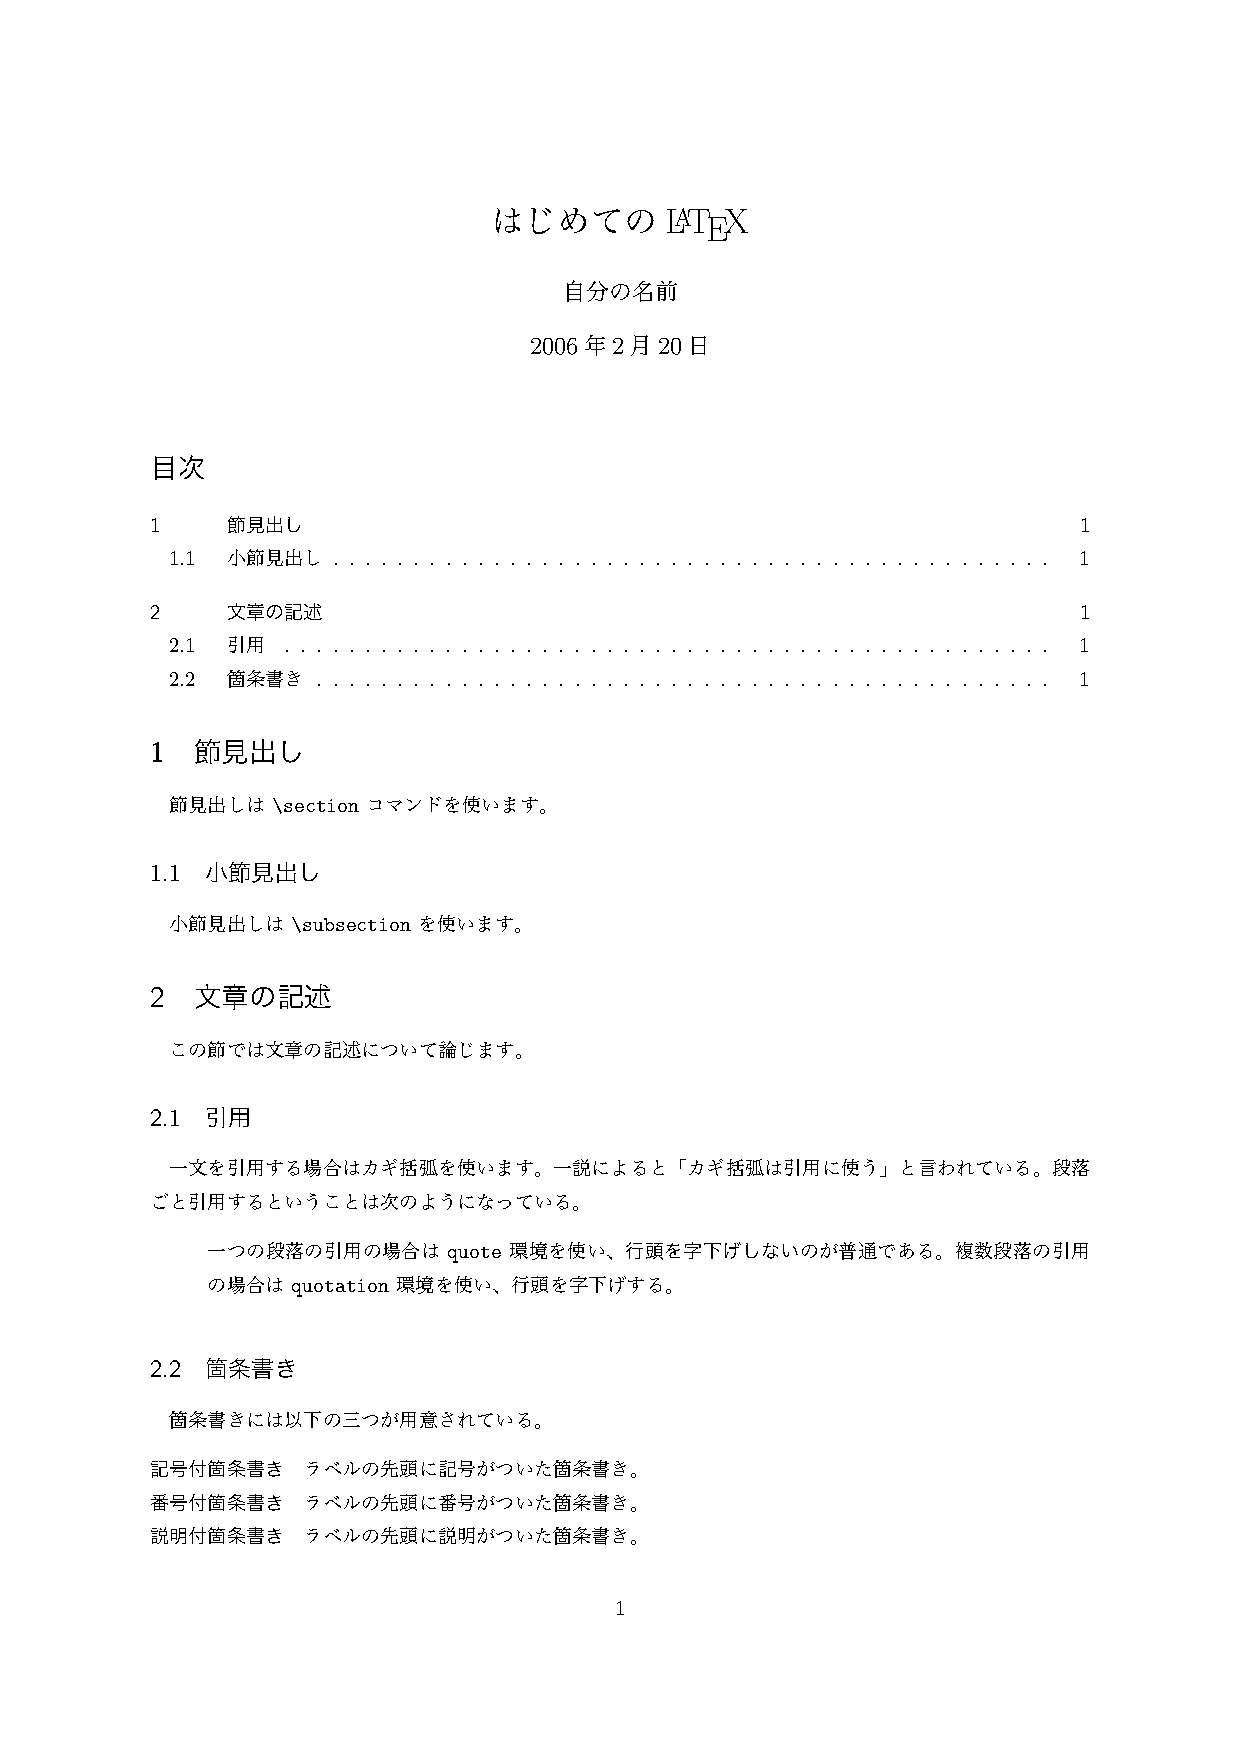
\includegraphics[clip,bb={0 0 595 842},width=\ffullwidth]
   {images/sample}\IOlabel}}
\caption{テキスト入力の出力例}\label{fig:sample}
\end{figure}

\end{Prob}



\section{書体について}\seclab{font}

%文字は意思伝達手段であって長いあいだに
%洗練された媒体です.怒りの意思を強く
%込めたいならば人は荒々しく文字を書く
%でしょうし,優しさを込めたいならば
%丸みを帯びた書き方になるでしょう.以
%上のような文字の形を書体と言います.
%%この章では{\LaTeX}で書体をどのように
%%扱っているのかを説明します.
%%文字はコミュニケーションツールです.覚書
%%などの個人的な文章を除き,文字は相
%%手に何かを伝えるために使われる媒体
%%,いわば道具です.日常的に文字とい
%%う道具を使っている私たちですが,普
%%段は音声,言葉による伝達が直感的な
%%ため,文字という道具の使い方を誤る
%%ときがあります.
%
%%怒っているときは荒々しい文字を書くと
%%そのときの感情が伝わりやすいでしょう,
%%これは正しい使い方です.怒っていると
%%きに弱々しい文字を書いても説得力があ
%%りません.これはあまり効果的な使い方
%%とは言えません.
%
%世の中にはこれらを書体というひとつの
%枠組みで整理しています.書体は読者に
%対して何らかのメッセージを分かりやす
%く伝えるために変更される場合がありま
%す.ですから書体を変更するということ
%には必ず意味があるべきなのです.むや
%みやたらに書体を変更しても逆に読者を
%混乱させます.また自分だけのルールで
%書体を変更しても読者には何の意味なの
%かが分かりませんので,一般的に使われ
%ている書体に関するルールを守るのもマ
%ナーです.
%
%{\LaTeX}は\Z{マークアップ}型のシステムな
%のでユーザが直接書体変更用の命
%令を使うことは本来ならば必要のないこ
%とだと思われます.以下のコマンドは直
%接使うのではなく新規に環境を定義して
%用いるのが望ましいでしょう.

\KY{文字} (\Z{character}) は\Z{意思伝達手段}であって,
長いあいだに洗練された\Z{媒体}です.怒りの意思を強く込
めたいならば人は荒々しく文字を書くでしょうし,優しさを
込めたいならば丸みを帯びた書き方になるでしょう.以上の
ような文字の形を\KY{書体} (\Z{typeface}) と呼びます.

世の中ではこれらを書体というひとつの枠組みで整理してい
ます.書体は読者に対して何らかのメッセージを分かりやす
く伝えるために変更される場合があります.ですから書体を
変更するという事には必ず意味があるべきなのです.むや
みやたらに書体を変更しても逆に読者を混乱させます.また
自分だけのルールで書体を変更しても読者には何の意味なの
かが分かりませんので,一般的に使われている書体に関する
ルールを守るのもマナーです.

{\LaTeX}は\Z{マークアップ}型のシステムなのでユーザが
直接書体変更用の命令を使う事は本来ならば必要のない事
だと思われます.以下のコマンドは直接使うのではなく新
規に環境を定義して用いるのが望ましいでしょう.


\subsection{文字の大きさの変更}
{\LaTeX}においては比較的簡単に文字の大きさを変える
事が可能ですが,文字は文書クラスオプションで指定
した基準の文字の大きさに応じて変更されます .文字
の大きさを変更したいときは\tabref{mojinookisa}
の宣言型のコマンド(\secref{ml:command}を参照)を
次のように使用します.

\begin{Syntax}
\texttt{\lb}\va{宣言} \va{文字の大きさを変えたい文字列}\texttt{\rb}
\end{Syntax}

\begin{table}[htbp]
\begin{center}
\caption{文字の大きさの変更}\tablab{mojinookisa}
\begin{tabular}{lll}
\TR
\Th{大きさ}       & \Th{命令}                 & \Th{出力例}\\
\MR
とても小さい & \Cmd{tiny}         & {\tiny 野鳥}\\
かなり小さい & \Cmd{scriptsize}   & {\scriptsize 花鳥}\\
小さい       & \Cmd{footnotesize} & {\footnotesize 雷鳥}\\
やや小さい   & \Cmd{small}        & {\small 白鳥}\\
普通         & \Cmd{normalsize}   & {\normalsize 飛鳥}\\
やや大きい   & \Cmd{large}        & {\large やちょう}\\
大きい       & \Cmd{Large}        & {\Large かちょう}\\
かなり大きい & \Cmd{LARGE}        & {\LARGE らいちょう}\\
とても大きい & \Cmd{huge}         & {\huge はくちょう }\\
特大         & \Cmd{Huge}         & {\Huge ひちょう}\\
\BR
\end{tabular}
\end{center}
\end{table}
%
\begin{table}[htbp]
\begin{center}
\caption{基準の文字の大きさによるコマンドの挙動の違い}
\tablab{moji:ookisatte}
 \begin{tabular}{lrrrl}
 \TR
 \Th{コマンド}\texttt\bs \Th{基準の大きさ}& 10\,pt  & 11\,pt   & 12\,pt &
 \Th{使用すべき要素}${}^{*}$\\
\MR
\Cmd{tiny}        & 5\,pt  & 6\,pt  &  6\,pt & 振り仮名\\
\Cmd{scriptsize}  & 7\,pt  & 8\,pt  &  8\,pt & \\
\Cmd{footnotesize}& 8\,pt  & 9\,pt  & 10\,pt & 索引・\Z{脚注}\\
\Cmd{small}       & 9\,pt  & 10\,pt & 11\,pt & 図表見出し\\
\Cmd{normalsize}  & 10\,pt & 11\,pt & 12\,pt & 小小節見出し・本文\\
\Cmd{large}       & 12\,pt & 12\,pt & 14\,pt & 小節見出し\\
\Cmd{Large}       & 14\,pt & 14\,pt & 17\,pt & 節見出し\\
\Cmd{LARGE}       & 17\,pt & 17\,pt & 20\,pt & \\
\Cmd{huge}        & 20\,pt & 20\,pt & 25\,pt & 部・章見出し番号\\
\Cmd{Huge}        & 25\,pt & 25\,pt & 25\,pt & 部・章見出し\\
\BR
 \end{tabular}
\\ {\small ${}^{*}$使用すべき要素は1段組での場合です.}
\end{center}
\end{table}
%
\begin{InOut}
そういえば,{\scriptsize これ}は小さい
文字だけど,{\Large こっち}は大きい
文字になってるね.
\end{InOut}
このような書体の大きさを変更するコマンドを
直接使うのは好ましくなく,きちんと\Z{マークアップ}付け
をするべきです.例えば\Z{強調}のために文字を大きく
したいのであれば新規に \cmd{kyocho} 命令を作ります.
\begin{InOut}
\newcommand\kyocho[1]{{\Large#1}}
\newcommand\Kyocho[1]{{\LARGE#1}}
だから\kyocho{ここは大事です}.それに
\Kyocho{ここはもっと大事}です.
\end{InOut}

\subsection{書体の変更}\seclab{ouyou:font}
%{\LaTeX}において書体の種類は
%\begin{description}
%\item[\Z{ファミリー}] デザイン上の系統の種類.
%\item[\Z{シリーズ}]   線の太さと文字幅の違いによる種類.
%\item[\Z{シェイプ}]   形状の変化の違いによる種類.
%\item[\Z{サイズ}]     フォントの大きさ.\zindind{フォント}{の大きさ}%
%\end{description}
%の四つに分けられます.サイズに関しては前述の通りです.

{\LaTeX}において書体の種類は次の四つに分けられます.
サイズに関しては前述の通りです.
\begin{description}
\item[\Z{ファミリー}] デザイン上の系統の種類.
\item[\Z{シリーズ}]   線の太さと文字幅の違いによる種類.
\indindz{幅}{文字の}%
\item[\Z{シェイプ}]   形状の変化の違いによる種類.
\item[\Z{サイズ}]     フォントの大きさ.\zindind{フォント}{の大きさ}%
\end{description}

文字の大きさや書体の種類を不必要に変更する事は,
逆に読者を混乱させるだけです.自分はきちんと使い分
ける事ができる,という方は\tabref{font:family}
の一覧から適切な書体を選んで,美しい文書を作成してく
ださい.%
\index{ローマン体}%
\index{サンセリフ体}%
\index{タイプライタ体}%
\index{ミディアム体}%
\index{ボールド体}%
\index{イタリック体}%
\index{スラント体}%
\index{スモールキャピタル体}%
\index{ファミリー!タイプライタ\zdash}%
\index{ファミリー!サンセリフ\zdash}%
\index{ファミリー!ローマン\zdash}%
\index{シェイプ!スモールキャピタル\zdash}%
\index{シェイプ!スラント\zdash}%
\index{シェイプ!イタリック\zdash}%
\index{シリーズ!ミディアム\zdash}%
\index{シリーズ!ボールド\zdash}%
%
% \textnormal, \normalfont の二つについての説明
% エンコーディングとファミリ,シリーズ,シェイプを標準に
%
\begin{table}[htbp]
\begin{center}
\caption{書体を変更するコマンド}\tablab{font:family}
\begin{tabular}{llll}
\TR
\Th{種類} & \Th{命令} & \Th{宣言} & \Th{出力} \\
\MR
ローマンファミリー     & \Cmd{textrm} & \Cmd{rmfamily} &
  \textrm{ABCabc}\\
サンセリフファミリー   & \Cmd{textsf} & \Cmd{sffamily} &
  \textsf{ABCabc}\\
タイプライタファミリー& \Cmd{texttt} & \Cmd{ttfamily} &
  \texttt{ABCabc}\\
\hline
ミディアムシリーズ     & \Cmd{textmd} & \Cmd{mdseries} &
  \textmd{ABCabc}\\
ボールドシリーズ       & \Cmd{textbf} & \Cmd{bfseries} &
  \textbf{ABCabc}\\
\hline
イタリックシェイプ     & \Cmd{textit} & \Cmd{itshape} &
  \textit{ABCabc}\\
スラントシェイプ       & \Cmd{textsl} & \Cmd{slshape} &
  \textsl{ABCabc}\\
スモールキャピタルシェイプ & \Cmd{textsc} & \Cmd{scshape} &
  \textsc{ABCabc}\\
\BR
\end{tabular}
\end{center}
\end{table}

%ファミリーとシリーズとシェイプはそれぞれ
%組み合わせて使うことができます.例えば
%\yo{セリフがなくて太くて傾いたフォント}という文字を
%出力したければ次のようにします.
%\begin{InOut}
%\textsf{\textbf{\textit{I like sushi.}}} 
%{\sffamily\bfseries\itshape I like sushi.} 
%\end{InOut}
%使用している基本書体によっては出力できない
%タイプもあります.
%\begin{InOut}
%\texttt{\textbf{Type writer and bold 
% extended?}} I like \textsc{small caps} and
%\textit{\textbf{bold italic}}. {\ttfamily
%\bfseries type writer and bold extended}
%\end{InOut}
%\K{書体のファミリーやシェイプなどを先に指定してから}
%大きさを変更します.%幾何学的にできないので当然のことです.
%\begin{InOut}
%{\Large\textbf Large Bold?} 成功.\\
%{\textbf\Large Bold Large?} 失敗.
%\end{InOut}
ファミリーとシリーズとシェイプはそれぞれ
組み合わせて使う事ができます.例えば
\yo{セリフがなくて太いフォント}という文字を
出力したければ次のようにします.
\begin{InOut}
\textsf{\textbf{Typeface}}
{\sffamily\bfseries Typeface} 
\end{InOut}
使用している基本書体によっては出力できない
タイプもあります.
\begin{InOut}
\texttt{\textit{Typewriter bold 
extended?}} \textsc{Small Caps}. 
\textit{\textbf{Bold italic}}. 
{\ttfamily \itshape typewriter 
bold extended.}
\end{InOut}
\emph{書体のファミリーやシェイプなどを先に指定してから
大きさを変更します}.
\begin{InOut}
{\Large\textbf Large Bold?} 成功\\
{\textbf\Large Bold Large?} 失敗
\end{InOut}

和文の書体は基本的には\Z{明朝体}と
\Z{ゴシック体}の二つしか用意されてい
ません\pp{\tabref{font:wa}}.これは
従来の和文組版で二つの書体しか使われな
かった名残です.現在の{\pLaTeX}で和文
の多書体を図る事はそれ程難しくあり
ません.ただ不用意に和文を多書体にして
も読者がそれに慣れていないと思われます
ので,徒に行わないほうが良いかもしれません.
\begin{table}[htbp]
\begin{center}
\caption{和文書体のファミリー}\tablab{font:wa}
  \begin{tabular}{llll}
\TR
 \Th{種類} & \Th{命令} & \Th{宣言} & \Th{出力}\\
\MR
% 明朝ファミリー& \Cmd{textmc} & 
%   \Cmd{mcfamily} & \textmc{永字八法って何ですか?}\\
% ゴシックファミリー&\Cmd{textgt} & 
%   \Cmd{gtfamily} & \textgt{永字八法って何ですか?}\\
 明朝ファミリー& \Cmd{textmc} & 
   \Cmd{mcfamily} & \textmc{永字八法とは何ですか?}\\
 ゴシックファミリー&\Cmd{textgt} & 
   \Cmd{gtfamily} & \textgt{永字八法とは何ですか?}\\
\BR
 \end{tabular}
\end{center}
\end{table}
\indindz{強調}{見出しの}\indindz{強調}{和文の}%%
\begin{InOut}
和文組版において明朝体は通常の文章の組
版,ゴシック体は\textgt{文章の強調に}
使われます.{\gtfamily 見出しも強調す
べき要素なのでゴシック体にするのが普通
です}.
\end{InOut}


\subsection{基本書体の変更}
フォントの大きさやファミリーなどを指定する命令は
分かりました.しかし,文書に使われている書体
そのものを変更するにはどうすれば良いのでしょうか.
実は普段何気なく{\LaTeX}で文書処理をしているときに
使われている欧文のフォントは\Person{Donald}{Knuth}が
デザインした\Z{Computer Modern}と呼ばれる
\KY{基本書体}になっています.この基本書体その
ものを変更するには基本書体を変更する定義がなされたマ
クロを読み込むか,自分で指定する必要があります.
数式に使われる数式書体にも基本的に{Computer Modern}
が使われます.フォントについては
\Hito{奥村}{晴彦}の文献~\cite{bibunsyo3}などを参照してく
ださい.本書では取り扱いません.
あえて言うならば%
\Person{Young}{Ryu}が作成した\Sty{txfonts}を使うのが
手軽ではないかと思います.標準配布のTimes系の
フォントを使うようにする\Sty{mathptmx}や,Palatino系
のフォントを使うようにする\Sty{mathpazo}よりも
\Sty{pxfonts}や\Sty{txfonts}という選択肢もあります(\secref{app:typeface}
を参照).


\section{文章の修正}
\zindind{原稿}{の校正}%
%このようにして基本的な文章構造を組み上げて,結果的に紙の上などに
%出力するわけですが,一発で完璧な文書になることはほとんどありません.
%何度も修正と加筆を繰り返し,最終的な論文に仕上がるものと思います.
%
%そのときに必要なのは文章の校正に関わる約束事です.
%{\LaTeX}ではほとんどの多くの処理を半自動的に行うので,
%普段は気にならない部分です.例えば半角英数字と全角の
%日本語とのあいだには四分空きといって,全角空白の4分の1の
%スペースを挿入したり,行の先頭に句読点があってはいけない
%という,行頭禁則処理の問題も{\LaTeX}\pp{{\pTeX}において}は
%半自動で行います.
%
%このような自動的な処理以外にもユーザ側の入力ミスにより修正
%が必要になる場合があります.その場合は1度作成した文章を校正
%記号~\cite{kumihan3}などを使って修正するのが良いでしょう.
%
%現在では文章はコンピュータ上ですべて組むことができるので,
%間違いを見つけたらその場ですぐに修正可能です. 紙に印刷し
%てチェックするという作業は非効率的かもしれません.コンピ
%ュータのモニター上と印刷した紙上の両者の特性を活かして文章
%を修正してください.
%文章作成上で注意すべき点として
%\begin{itemize}
% \item 1文を長くしすぎていないか.
% \item である調で統一されているか.
% \item 修飾語の関係をはっきりしているか.
% \item 同音異義語などの間違いはないか.
% \item 段落の区切り,章の区切りは明確か.
%\end{itemize}
%などが挙げられます.

このようにして基本的な文章の論理構造を組み上げて,結果的に紙
の上などに出力するわけですが,一発で完璧な文書になる事はほ
とんどありません.何度も修正と加筆を繰り返し,最終的な論文に
仕上がるものと思います.

そのときに必要なのは文章の校正に関わる約束事です.{\LaTeX}で
はほとんどの多くの処理を半自動的に行うので,普段は気にならな
い部分です.例えば半角の英数字と全角の日本語とのあいだには
\Z{四分空き}といって,全角空白の4分の1のスペースを挿入したり,
行の先頭に句読点があってはいけないという,行頭\Z{禁則処理}の
問題も{\LaTeX}\pp{{\pTeX}において}は半自動で行います.
% 対処するという表現の方が適切ではないだろうか.

\indindz{記号}{校正}%
\index{間違いの修正}%
このような自動的な処理以外にもユーザ側の入力ミスにより修正
が必要になる場合があります.その場合は1度作成した文章を\Z{校正}
記号~\cite{NES1999}などを使って修正するのが良いでしょう.


現在では文章はコンピュータ上ですべて組む事ができるので,
間違いを見つけたらその場ですぐに修正可能です. 紙に印刷し
てチェックするという作業は非効率的かもしれません.コンピ
ュータのモニター上と印刷した紙上の両者の特性を活かして文章
を修正してください.
文章作成~\cite{HO2004,HO2002,KK1981}上で注意すべき点として
以下の項目などが挙げられます.
\begin{itemize}
 \item 1文を長くしすぎていないか.
 \item である調で統一されているか.
 \item 修飾語の関係をはっきりしているか.
 \item 同音異義語などの間違いはないか.
 \item 段落の区切り,章の区切りは明確か.
\end{itemize}


%\subsection{スペルチェック}
%欧文の文書の場合はスペルミスをチェックできるプログラムが
%いくつかあります.

\subsection{構文チェック\zdash\Y{syntonly}}
{\LaTeX}の原稿を書いていると,コマンド構文の記述ミスをして
しまう事があります.括弧が足りないとか,大文字と小文字を書き間違えている
などです.
\Person{Frank}{Mittelbach}と\Person{Rainer}{Sch\"opf}が作成した
\Sty{syntonly}を使うと,自分の記述が間違っていないか,実際の出力をせずに
構文のチェックだけを行うようにできます.
%
\Cmd{syntaxonly}命令をプリアンブルに記述します.\Sty{syntonly}パッケージ
を読み込んだだけでは何も起こりません.
%
構文だけをチェックするので通常のDVI出力を伴うタイプセットよりも処理が速
いと思います.

\begin{InTeX}
\documentclass{jarticle}
\usepackage{syntonly}
\syntaxonly
\begin{document}
I like {\LaTex}.%これはエラーになります.
\end{document}
\end{InTeX}


\section{クラスとパッケージ}\seclab{class}
{\LaTeX}は\Z{マークアップ}方式を採用した言語なので\Z{書式}と内容は
分離されるのが一般的です.そこで\Z{クラス}\pp{\Z{class}}と
\Z{パッケージ}\pp{\Z{package}}という二つのファイルを使う
ようになっています.

%さて,クラスやパッケージという用語が出てきましたが,簡単
%に説明しましょう.昔の話は置いといて\pp{{\LaTeX2.09}},
{\LaTeX}では文書の書式を決定するためにクラスというもの
を宣言します.クラスは\Z{ドキュメントクラス}とか
\Z{文書クラス}などと呼ばれています.また,便利な機能%
\zindind{マクロ}{パッケージ}%
を集めたものを\K{パッケージ}と呼びます.パッケージは\K{マクロパッケージ}
とか,ただ単に\KY{マクロ}などと呼ばれます.

そうして,{\LaTeX}の原稿\pp{\Z{ソースファイル}}では必ず文
書の先頭に
\begin{Syntax}
\cmd{documentclass}\opa{オプション$,\ldots$}\pa{クラス}\\ 
\cmd{usepackage}\opa{オプション$,\ldots$}\pa{パッケージ}
%\cmd{documentclass}\opa{オプション}\pa{クラス}\\ 
%\cmd{usepackage}\opa{オプション}\pa{パッケージ}
\end{Syntax}
のような記述をして,文書の書式を大雑把に決定します.

%例えば,日本語の小規模の画像を含み,書体の大きさが11ポイントで
%\Z{2段組}の記事を書こうと思えば
例えば,本文が日本語で画像を含み,書体の大きさが11ポイントで
\Z{2段組}の記事を書こうと思えば次のように原稿中で宣言します.

\begin{InTeX}
\documentclass[twocolumn,11pt]{jarticle}
\usepackage[dvips]{color}
\usepackage[dvips]{graphicx}
\end{InTeX}

使用するクラスの中にはオプションが
存在し,上記のように2段組のために\option{twocolumn}やフォントの
大きさを指定するために\option{11pt}というオプションを指定します.
また衝突の起きない限り,複数のパッケージを使う事を
同時に宣言する事もできます.

\begin{InTeX}
\documentclass[twocolumn,11pt]{jarticle}
\usepackage[dvips]{graphicx,color}
\end{InTeX}

クラスとパッケージを明確に区別するために
クラスの\Z{拡張子}には\exten{cls}を,
パッケージの拡張子には\exten{sty}を付けるようにします.

\subsection{標準的なクラス}\seclab{01pregame:sec:classes}

\indindz{クラス}{標準的な}%
{\LaTeX}や{\pLaTeX}の範囲内で提供されている標準的なクラスを
紹介します.クラスファイルは\Va{classes}{dtx}と
\Va{classes}{ins}という二つのファイルで配布される事が多い
ようです.

あるクラスが何からインストールできるのかは,すでにでき
上がっているクラスファイル\Va{classes}{cls}が存在すれば
そのファイルの先頭部分に次のような記述があります.

\begin{InTeX}
%% This is file `class.cls',
%% generated with the docstrip utility.
%% The original source files were:
%% classes.dtx  (with options: `option')
\end{InTeX}

オリジナルのソースファイルは
オプションに\option{`option'}を指定してファイル名が
\Va{classes}{dtx}です,と説明してくれていますので
Unix系OSならば
\begin{InTerm}
  \type{find /usr/local/share/texmf/ -name classes.dtx}
\end{InTerm}
などでそのファイルを検索できるでしょう.WindowsやMacintosh
はファイルの検索の機能があると思いますので,そちらを使えば
良いでしょう.そのようにして検索した場所に\Va{classes}{dtx}や
\Va{classes}{ins}が存在します.そのファイルがある場所に移動して
%\begin{InTerm}
  \type{platex classes.dtx}
%\end{InTerm}
とすればそのクラスの仕様書を見る事ができます.さらに
%\begin{InTerm}
  \type{platex classes.ins}
%\end{InTerm}
とするとそのクラスを導入する事ができます.このような操作をすると
\Sty{DocStrip}というマクロが適切にファイルを処理します.
例えばファイル\Fl{classes.ins}をこのように処理すると,
\Fl{article.cls},\Fl{report.cls},\Fl{book.cls},\Fl{bk10.clo},
\Fl{bk11.clo},\Fl{bk12.clo},\Fl{size10.clo},\Fl{size11.clo},
\Fl{size12.clo}という九つのファイルが生成されます.

日本語を含まないような文書には欧文専用のクラスが使用できます.
それぞれどのような文書を作成したいかによって何を用いるかが
分かれます.標準では以下の欧文用のクラスが使えます.
\begin{namelist}{xxxx}
\item[\Cls{article}] 小規模の記事を作成するためのクラス.
	\Fl{classes.dtx}や{\COMP}に詳しい仕様が書かれている.
\item[\Cls{report}]  報告書を作成するためのクラス.
	同じく\Fl{classes.dtx}や{\COMP}に詳しい仕様が書かれている.
\item[\Cls{book}]    書籍を作成するためのクラス.
	同じく\Fl{classes.dtx}や{\COMP}に詳しい仕様が書かれている.
\item[\Cls{slides}]  スライドを作成するためのクラス.
	\Fl{slides.dtx}に詳しい仕様が書かれている.
\item[\Cls{proc}]    \cls{article}をベースに議事録などを%
	作成するためのクラス.
	\Fl{proc.dtx}に詳しい仕様が書かれている.
%\item[\cls{ltxdoc},\cls{ltxguide},\cls{ltnews}] 
%	開発者用のクラスファイル.一般ユーザにはあまり縁のないもの.
%	それぞれ,\fl{ltxdoc.dtx},\fl{ltxguide.dtx},
%	\fl{ltnews.dtx}に詳しい仕様が書かれている.
%\item[\cls{minimal}] {\LaTeX}を取り扱う上で最小限の定義を
%したクラスファイル.このクラスを元に自分流のクラスを新たに
%開発することもできる.
\end{namelist}
以上の\cls{article},\cls{report},\cls{book}の三つをまとめて
\Cls{classes}と呼ぶ事があります.

日本語の文書では,標準で以下のクラスが使えます.
\begin{namelist}{xxxxx}
\indindz{クラス}{小規模な文書用の}
\item[\Cls{jarticle}] 小規模の日本語の記事を作成するためのクラス.
\indindz{クラス}{報告書用の}
\item[\Cls{jreport}]  日本語の報告書を作成するためのクラス.
\indindz{クラス}{書籍用の}
\item[\Cls{jbook}]    日本語の書籍を作成するためのクラス.
\item[\Cls{tarticle}] 縦書きの小規模の日本語の記事を作成するためのクラス.
\item[\Cls{treport}]  縦書きの日本語の報告書を作成するためのクラス.
\item[\Cls{tbook}]    縦書きの日本語の書籍を作成するためのクラス.
\end{namelist}
以上の\cls{jarticle},\cls{jreport},\cls{jbook}の三つをまとめて
\Cls{jclasses}と呼ぶ事があります.

\subsection{クラスオプション}\seclab{classopt}
ドキュメントクラス\pp{文書クラス}にはもう少し詳細な
設定を行う事ができます.\cmd{documentclass}の任意引数として
記述します.多くのクラスファイルでは次の\Z{クラスオプション}が
使えると思います.
%\begin{description}
%
%\item[\Z{文字サイズ}\av{\Optionlist{10pt,11pt,12pt}}]
%原稿で基本となる文字の大きさを決めます.この文字サイズを
%基準としてさまざまなパラメータが設定されます.標準は
%\option{10pt}.
%
%\item[\Z{用紙サイズ}\av{\Optionlist{a4paper,a5paper,b5paper,letterpaper}}]
%原稿の用紙の大きさを指定します.\index{用紙!\zdash のサイズ}%
%\index{用紙!\zdash の大きさ}%
%和文の場合はこの他に\Optionlist{b4paper,a4j,a5j,b4j,b5j}などです.
%\sty{geometry}パッケージや\cls{jsclasses}を使うと選択の幅が
%広がります.
%
%\item[\Z{用紙方向}\av{\Option{landscape}}]
%用紙を横置きにします.標準は縦置きです.\index{用紙!\zdash の方向}
%
%\item[\Z{印刷面}\av{\Optionlist{oneside,twoside}}]
%用紙の片面\pp{\option{oneside}}だけに印刷するか
%それとも両面\pp{\option{twoside}}に印刷するかを指定します.
%\item[\Z{段組}\av{\Optionlist{onecolumn,twocolumn}}]
%%\ex{段組}{1段組}\index{段組}{2段組}%
%\Z{1段組}\pp{\option{onecolumn}}にするか\Z{2段組}\pp{\option{twocolumn}}
%にするかを指定します.
%
%\indindz{表題}{独立ページの}\indindz{表題}{同ページの}\indindz{ページ}{表題}
%\item[\Z{表題}\av{\Optionlist{titlepage,notitlepage}}]
%表題を独立して出力する\pp{\option{titlepage}}か,
%同じページに出力する\pp{\option{notitlepage}}かという表題の
%レイアウトを指定します.
%
%\item[{数式の位置}\av{\Option{fleqn}}]
%\zindind{数式}{の位置}%	   
%別行数式の位置を左揃えに指定します.標準は中央揃えです.
%	
%\item[{数式番号の位置}\av{\Option{leqno}}]
%\zindind{数式}{番号の位置}%
%数式番号の位置を左側に指定します.標準は右側です.
%	
%\item[\Z{ドラフト}\av{\Optionlist{draft,final}}]
%文書の領域をはみ出してしまった箇所に印をつけるかどうか.
%執筆途中で印刷するときにはドラフトモードにする.
%ドラフトモードの\option{draft},
%原稿が完成したら\option{final}に変更する.
%標準は\option{final}.
%
%\item[\Z{左右起し}\av{\Optionlist{openright,openany}}]
%\cls{(j)report}や\cls{(j)book}において章などの開始ページの
%指定をする.常に奇数ページで起こす\pp{\option{openright}}か,
%どちらからでも起こす\pp{\option{openany}}かを設定する.
%\cls{(j)report}の標準は\option{openany}.
%\cls{(j)book}の標準は\option{openright}.
%\end{description}

\begin{description}
\item[{文字サイズ}\av{\Optionlist{10pt,11pt,12pt}}] 
\zindind{文字}{サイズ}%
\zindind{原稿}{の文字サイズ}%
原稿で基本となる文字の大きさを決めます.この文字サイズを
基準としてさまざまなパラメータが設定されます.標準は
\option{10pt}.

\item[{用紙サイズ}\av{\Optionlist{a4paper,a5paper,b5paper,letterpaper}}]
原稿の用紙の大きさを指定します.
\index{用紙!\zdash のサイズ}%
\index{用紙!\zdash の大きさ}%
\zindind{原稿}{の用紙サイズ}%
和文の場合はこの他に\Optionlist{b4paper,a4j,a5j,b4j,b5j}などです.
\sty{geometry}パッケージや\cls{jsclasses}を使うと選択の幅が
広がります.

\item[{用紙方向}\av{\Option{landscape}}]
用紙を横置きにします.標準は縦置きです.\index{用紙!\zdash の方向}

\item[\Z{印刷面}\av{\Optionlist{oneside,twoside}}]
用紙の片面\pp{\option{oneside}}だけに印刷するか
それとも両面\pp{\option{twoside}}に印刷するかを指定します.
\item[\Z{段組}\av{\Optionlist{onecolumn,twocolumn}}]
\indindz{段組}{1}\indindz{段組}{2}%
\Z{1段組}\pp{\option{onecolumn}}にするか\Z{2段組}\pp{\option{twocolumn}}
にするかを指定します.

\indindz{表題}{独立ページの}\indindz{表題}{同ページの}\indindz{ページ}{表題}
\item[{表題}\av{\Optionlist{titlepage,notitlepage}}]
表題を独立して出力する\pp{\option{titlepage}}か,
同じページに出力する\pp{\option{notitlepage}}かという表題の
レイアウトを指定します.

\item[{数式の位置}\av{\Option{fleqn}}]
\zindind{数式}{の位置}%	   
別行数式の位置を左揃えに指定します.標準は中央揃えです.
	
\item[{数式番号の位置}\av{\Option{leqno}}]
\zindind{数式}{番号の位置}%
数式番号の位置を左側に指定します.標準は右側です.
	
\item[\Z{ドラフト}\av{\Optionlist{draft,final}}]
\indindz{原稿}{ドラフト段階の}%
\indindz{原稿}{執筆段階の}%
執筆途中で印刷するときに\option{draft}オプションを付けると,
文書幅の領域をはみ出してしまった箇所に印が付いてくれます.
原稿が完成したら\option{final}に変更します.標準は\option{final}です.

\item[\Z{左右起し}\av{\Optionlist{openright,openany}}]
\cls{(j)report}や\cls{(j)book}において章などの開始ページの
指定をします.常に奇数ページで起こす\pp{\option{openright}}か,
どちらからでも起こす\pp{\option{openany}}かを設定します.
\cls{(j)report}の標準は\option{openany}.
\cls{(j)book}の標準は\option{openright}.
\end{description}


最近では,\Hito{奥村}{晴彦}が管理している
\Cls{jsclasses}というクラスファイル群に定評があります\footnote{\webJsclasses}.
このクラス群を導入すると
\begin{namelist}{xxxxxx}
\item[\Cls{jsarticle}]	小規模の日本語の記事を作成するためのクラス.
\item[\Cls{jsbook}]	日本語の書籍や報告書を作成するためのクラス.
\item[\Cls{jspf}]	某学会誌用のクラス.
\end{namelist}
の三つが使用できます.これらのクラスで指定できる
クラスオプションが\cls{jclasses}に追加されて
います\footnote{\cls{(j)classes}で定義されていたいくつかの
クラスオプションが実装されていません.}.
以上の\cls{jsarticle},\cls{jsbook},\cls{jspf}の三つをまとめて
\Cls{jsclasses}と呼びます.

\begin{description}
\item[\Z{文字サイズ}]\av{\Optionlist%
   {9pt,10pt,11pt,12pt,14pt,17pt,20pt,21pt,25pt,30pt,36pt,43pt,12Q,14Q}}
\item[\Z{用紙サイズ}]\av{\Optionlist%
   {a4paper,a5paper,a6paper,b5paper,b4paper,a4j,a5j,b4j,b5j,a4var,b5var}}
\item[言語の指定]\av{\Option{english}}
  欧文用の見出しの定義と行送りになります.
\item[用紙サイズ情報] \av{\Option{papersize}} 
  用紙サイズの情報をデバイスドライバに渡すようにします.
\item[レポート作成] \av{\Option{report}} 
  \Z{レポート作成}用に \cmd{chapter} 命令を使う事ができます.
  \cls{jsbook} では左右起し等に関する設定が変わります.
\end{description}

\subsection{標準で使用できるパッケージ}\seclab{01pregame:sec:stdmacro}
{\LaTeX}を導入すると一緒に添付される標準的なパッケージがあります.
これらはプリアンブル部分に次のようにすると使用可能になります.
\begin{Syntax}
\C{usepackage}\opa{オプション}\pa{パッケージ}
\end{Syntax}

各パッケージの詳細な説明書が読みたいときは
\begin{InTerm}
   \type{platex filename.dtx}
\end{InTerm}
とすれば\Va{filename}{dvi}が作成されます\footnote{最近の\TeX 環境
では \underline{\str{texdoc }\va{パッケージ名}}等とすればマニュアル
が表示されます.}.索引の作成や
目次の作成,相互参照の解決などをすれば完全なDVIファイルが
完成します.各ソースファイルへの検索パスがなければ
該当する\Va{filename}{dtx}を検索する事はできません.
{Windows}ならばファイルの検索,Unix系OSならば\prog{find}コマンド
などで探してください.大抵は{\LaTeX}をインストールした
ディレクトリ\pp{フォルダ}の下\qu{\fl{\$texmf/tex/latex/base}}にあります.
%\begin{namelist}{xxxxxx}
%\item[\Sty{alltt}]	\Env{alltt}環境を提供するためのマクロ.
%この環境内では\verb|\|,\verb|{|,\verb|}|が通常通りの命令として
%解釈され,{\LaTeX}のコマンドなどが使える.\Fl{alltt.dtx}から
%生成される.
%\item[\Sty{doc}]	パッケージファイルが必要とするマクロ.
%\Fl{doc.dtx}から生成される.
%\item[\Sty{exscale}]	\Fl{exscale.dtx}
%\item[\Sty{fontenc}]	\Fl{fontenc.dtx}
%\item[\Sty{graphpap}]	\Fl{graphpap.dtx}
%\item[\Sty{ifthen}]	\Fl{ifhten.dtx}
%\item[\Sty{inputenc}]	\Fl{inputenc}
%\item[\Sty{latexsym}]	\Fl{latexsym}
%\item[\Sty{makeidx}]	索引作成用のマクロ.
%\Fl{makeindx.dtx}から生成される.
%\item[\Sty{newlfont}]	\Fl{newlfont.dtx}
%\item[\Sty{oldlfont}]	\Fl{oldlfont.dtx}
%\item[\Sty{syntonly}]	実際の出力をせずに,構文解析のみを行うマクロ.
%\Fl{syntonly.dtx}から生成される.
%\item[\Sty{tracefnt}]	文書中で使用される書体の情報を詳しく
%表示するためのマクロ.\Fl{ltfsstrc.dtx}から生成される.
%\end{namelist}
%これらのファイルについて詳しくは\wasyo{\LMANUAL}や
%\wasyo{\COMP}を見てください,だそうです.まあ,それだけでは
%少し寂しいので,何か有益な{\LaTeX}に
%関するウェブページがないか探すことになるわけですが,
%\wasyo{\LMANUAL}を
%超えるものは存在しないのが現状です.\yo{作者より詳しくて分かりやすい
%文書がウェブページに存在したら洒落にならんわぁ.}という言葉が,
%またどこからともなく聞こえてきたのでこの辺で説明を終わります.

{\LaTeX}がコンピュータに導入されているならば以下の応用的な
マクロやソフトウェアが同封されている事でしょう.
これらのファイルは欧文の文書を作成するうえでは必須のものと
されています.%日本語の文書のみを作成するならば,
%いくつかのマクロやソフトウェアは必要ないでしょう.

\begin{description}
\item[{\Prog[AmSLaTeX]{\AmSLaTeX}}] 
  \Z{米国数学会}\pp{\Z{American Mathematical Society}}が
  提供しているソフトウェア並びにパッケージ.
  \Prog[AmSTeX]{\AmSTeX}という\prog{\TeX}用を{\LaTeX}でも使えるように
  したもの.マクロ,フォントなどを総称した呼び名が
  {\AmSLaTeX}で,\LaTeX でのパッケージの名前は\Sty{amsmath}と言います.
  \secref{amsmath}で紹介しています.
  \indindz{マクロ}{数学系の}%

\item[\Sty{babel}] 多言語を{\LaTeX}で扱うためのマクロ.
  このマクロを日本語と共存させるためには少々工夫が必要.
  詳しい情報は\appref{webpage}を参照してください.

%\item[\Sty{cyrillic}] キリルフォントで文書を作成するときに必要になるマクロ群.

\item[\Sty{graphicx}] 画像の挿入や加工などを担うマクロ.
同時に\Sty{color}というマクロも含まれます.これはデバイス依存の
機能で環境により出力が異なる事があります.
\secref{gazou}で紹介しています.

%\item[\Sty{psnfss}] Everything you need for typesetting with a large range of Type 1 fonts.
\item[\Sty{tools}] {\LaTeX\,3}プロジェクトチームによって提供される
標準からはこぼれたマクロ.

\end{description}

%これらのマクロについては少なくとも{\COMP}か{\LMANUAL}
%に記述されていることが保証されています.

{\LaTeX\,3}プロジェクトチームによって提供される\sty{tools}
は\qu{\fl{\$texmf/tex/latex/tools}}に置かれており,
その内訳は以下のとおりです.
%\begin{namelist}{xxxxxxxx}
%\item[\Y{array}] 	\Env{array}や\Env{tabular},\Env{tabular*}
%のような表や行列を拡張した環境を使うことができるマクロ.
%\item[\Y{calc}] 		{\LaTeX}での計算を楽にするマクロ.
%\item[\Y{dcolumn}] 	表や行列の環境で\Z{小数点}などを揃えるためのマクロ.
%\item[\Y{delarray}] 	行列で括弧付けを容易にするためのマクロ.
%\item[\Y{hhline}] 	表や行列で複雑な罫線を簡単に引くことができる
%マクロ.
%\item[\Y{longtable}] ページをまたぐような長いなが〜い表を
%作るときに使うマクロ.
%\item[\Y{tabularx}] 	通常の\env{tabular}環境よりも幅に関して
%柔軟な表を作るためのマクロ.
%\item[\Y{afterpage}] \Cmd{clearpage}の拡張版のような
%\Cmd{afterpage}が使えるマクロ.
%\item[\Y{bm}] 		数式中で太字を簡単に使うようにするためのマクロ.
%\item[\Y{enumerate}] \Env{enumerate}環境を拡張するためのマクロ.
%\item[\Y{fontsmpl}] 	任意のフォントの一覧を表示するためのマクロ.
%\item[\Y{ftnright}] 	2段組で全ての{脚注}を右側に表示するマクロ.
%\indindz{脚注}{2段組での}
%\item[\Y{indentfirst}] \Cls{jarticle}や\Cls{jreport}などの
%標準的なクラスで,章\pp{\Cmd{chapter}}や節\pp{\Cmd{section}}の直後の段落でも
%字下げを行うようにするマクロ.通常は字下げしないように設定されている
%ので,和文文書を作成しているときはいつでも読み込むようにすれば良い.
%\indindz{字下げ}{見出し直後の}%
%\zindind{見出し}{の直後}%%
%\item[\Y{layout}] 	現在の文書のページレイアウトを表示するマクロ.
%\item[\Y{multicol}] 	他段組を実現するためのマクロ.
%%\item[\Y{rawfonts}] 	
%%\item[\Y{somedefs}] 	
%\zindind{相互参照}{のラベルの表示}%
%\item[\Y{showkeys}] 	\Cmd{label},\Cmd{ref},\Cmd{cite}などの
%相互参照のラベル名\pp{keys}を表示するためのマクロ.
%\item[\Y{theorem}] 	定義型環境を簡単に宣言するためのマクロ.
%\item[\Y{varioref}] 	相互参照をしやすくするためのマクロ.
%\item[\Y{verbatim}] 	\Env{verbatim}環境を拡張するためのマクロ.
%\indindz{相互参照}{別の文書との}%
%\item[\Y{xr}] 		別の文書とでも相互参照できるようにするためのマクロ.
%\item[\Y{xspace}] 	文中で使われるようなマクロに適切な
%			空白の挿入などを行うマクロ.
%\end{namelist}		
\begin{namelist}{xxxxxxxx}
\item[\Sty{array}] 
  \Env{array}や\Env{tabular},\Env{tabular*}
  のような表や行列を拡張した環境を使う事ができるマクロ.
\item[\Sty{calc}]
  \latexno{での計算}
  {\LaTeX}での計算を楽にするマクロ.
  \secref{calc}で紹介しています.
\item[\Sty{dcolumn}] 
  \zindind{行列}{中の小数点}%
  \zindind{表}{中の小数点}%
  表や行列の環境で\Z{小数点}などを揃えるためのマクロ.
  \secref{dcolumn}で紹介しています.
\item[\Sty{delarray}] 
  \zindind{行列}{に付ける括弧}%
  \zindind{括弧}{のある行列}%
  行列で括弧付けを容易にするためのマクロ.
  \secref{math:array}で紹介しています.
\item[\Sty{hhline}] 
  \zindind{表}{の罫線}%
  \zindind{行列}{の罫線}%
  表や行列で複雑な罫線を簡単に引く事ができるマクロ.
\item[\Sty{longtable}] 
  \indindz{表}{長い}
  \indindz{表}{ページを跨ぐ}
  ページをまたぐような,\Z{非常に長い表}を作るときに使うマクロ.
  \secref{longtable}で紹介しています.
\item[\Sty{tabularx}] 	
\indindz{幅}{表の}%
  通常の\env{tabular}環境よりも幅に関して
  柔軟な表を作るためのマクロ.
 \secref{tabularx}で紹介しています.
\item[\Sty{afterpage}] 
 \C{clearpage}の拡張版のような \C{afterpage}が使えるマクロ.
%これはページ数が足りなかった時の保険として
\item[\Sty{bm}] 
  \zindind{数式}{中の太字}%
  \indindz{太字}{数式中の}%
  数式中で太字を簡単に使うようにするためのマクロ.
  \secref{bm}で紹介しています.
\item[\Sty{enumerate}] 
  \Env{enumerate}環境を拡張するためのマクロ.
  \secref{enumerate}で紹介しています.
%\item[\Sty{fontsmpl}] 	
%  任意のフォントの一覧を表示するためのマクロ.
\item[\Sty{ftnright}]
  2段組で全ての{脚注}を右側に表示するマクロ.
  \indindz{脚注}{2段組での}
\item[\Sty{indentfirst}] \Cls{jarticle}や\Cls{jreport}などの
標準的なクラスで,章\pp{\cmd{chapter}}や節\pp{\cmd{section}}の直後の段落でも
字下げを行うようにするマクロ.通常は字下げしないように設定されている
ので,和文文書を作成しているときはいつでも読み込むようにすれば良い.
\indindz{字下げ}{見出し直後の}%
\zindind{見出し}{の直後}%%
\secref{indentfirst}で紹介しています.
\item[\Sty{layout}]
  \zindind{文書}{のページレイアウト}
  現在の文書の{ページレイアウト}を表示するマクロ.
  \secref{layout}で紹介しています.
\item[\Sty{multicol}] 	
  \Z{多段組}を実装するためのマクロ.
  \secref{multicol}で紹介しています.
%\item[\Sty{rawfonts}] 	
%\item[\Sty{somedefs}] 	
\item[\Sty{showkeys}]
  \zindind{相互参照}{のラベルの表示}%
  \Cmd{label}, \Cmd{ref}, \Cmd{cite}などの
  相互参照のラベル名\pp{keys}を表示するためのマクロ.
  \secref{showkeys}で紹介しています.
\item[\Sty{theorem}] 	
  \Z{定理}型環境を簡単に宣言するためのマクロ.
  \secref{theorem}で紹介しています.
\item[\Sty{varioref}] 	
 \zindind{相互参照}{の簡略化}%
  相互参照をしやすくするためのマクロ.
\item[\Sty{verbatim}] 	
  \Env{verbatim}環境を拡張するためのマクロ.
% 入れても良い気がするが.
\item[\Sty{xr}]
  \indindz{相互参照}{別の文書との}%
  別の文書とでも相互参照できるようにするためのマクロ.
% これはあるかなぁ.
\item[\Sty{xspace}]
  \zindind{コマンド}{の後の空白文字}
  文中で使われるようなマクロに適切な空白の挿入などを行うマクロ.
  \secref{xspace}で紹介しています.
\end{namelist}		


%\endinput

